%=================================================================
% Grammar / Tokenization paper (grammarpaper -> two_paper_split).
% Reformatted to MDPI Sensors. Compile: pdflatex; bibtex grammar_paper; pdflatex x2.
%=================================================================
\documentclass[sensors,article,submit,moreauthors,pdftex]{Definitions/mdpi}

%=================================================================
% MDPI frontmatter
\firstpage{1}
\makeatletter
\setcounter{page}{\@firstpage}
\makeatother
\pubvolume{1}
\issuenum{1}
\articlenumber{0}
\pubyear{2026}
\copyrightyear{2026}
\history{}

%=================================================================
% Packages (mdpi.cls already loads: amsmath, amsthm, booktabs, enumitem,
% fancyhdr, tikz, xcolor[table], natbib, etc. and defines Theorem/Definition/...)
\usepackage{amssymb}
\usepackage{multirow}
\usepackage{subcaption}
\usepackage{graphicx}
\usepackage{float}
\usepackage{xcolor}
\usepackage{listings}
\usepackage{algorithm}
\usepackage{algpseudocode}
\usetikzlibrary{arrows.meta, positioning, decorations.pathreplacing, calc}
\graphicspath{{../}{../figures/}}

\lstset{
  basicstyle=\ttfamily\small,
  breaklines=true,
  frame=single,
  backgroundcolor=\color{gray!10},
  numbers=none,
  xleftmargin=2mm,
  framexleftmargin=2mm
}

% Convenience macros
\newcommand{\ie}{\textit{i.e.}}
\newcommand{\eg}{\textit{e.g.}}
\newcommand{\etal}{\textit{et al.}}
\newcommand{\etc}{\textit{etc.}}

% MDPI back-matter macros not present in the local (older) mdpi.cls.
\providecommand{\institutionalreview}[1]{\medskip\noindent\textbf{Institutional Review Board Statement:} #1\par}
\providecommand{\informedconsent}[1]{\medskip\noindent\textbf{Informed Consent Statement:} #1\par}
\providecommand{\dataavailability}[1]{\medskip\noindent\textbf{Data Availability Statement:} #1\par}

%=================================================================
% Title
\Title{Formalizing G-Code for Language Models: Grammar-Aware Hierarchical Tokenization of CNC Milling Toolpaths}

\newcommand{\orcidauthorA}{0009-0009-0292-9706}

\Author{Stephen S. Eacuello $^{1,}$*\orcidA{}, Romesh S. Prasad $^{1}$ and Manbir S. Sodhi $^{1}$}

\AuthorNames{Stephen S. Eacuello, Romesh S. Prasad and Manbir S. Sodhi}

\address{%
$^{1}$ \quad Department of Industrial Systems Engineering, University of Rhode Island, Kingston, RI 02881, USA}

\corres{Correspondence: seacuello@uri.edu}

\abstract{
G-code controls nearly all CNC manufacturing, yet standard tokenizers fail on it: 97\% of a single workpiece's vocabulary entries are numeric coordinates, the vocabulary scales with part geometry, and subword splitting destroys semantic units. We formalize G-code toolpath syntax as a regular grammar and propose a three-level tokenization framework (a finite-state grammar, hierarchical type/identity/value decomposition, and digit-by-digit numeric prediction) that fixes the structural vocabulary at 19 tokens regardless of geometry. A design-space analysis over three properties (bounded vocabulary, lossless coordinate representation, value-level grammar validity) shows by case analysis that of the three dominant tokenizer classes, only structured digit decomposition provides all three simultaneously. We verify every cell of the design-space table empirically. Across seven tokenizer families on 120 CNC milling files, only digit-decomposed and character-level tokenizers achieve near-zero held-out OOV ($\le\!0.002\%$). Decoders trained with standard whitespace-pre-tokenized BPE reach $0.00 \pm 0.00\%$ free-generation grammar validity through decode-time whitespace reinsertion; a byte-level BPE control recovers to $97.1\%$. Grammar masking shifts type-transition distributions by only $0.005 \pm 0.003$ nats. Under 5-fold cross-validation the hierarchical decoder reaches 94.7\% token accuracy and 84.4\% sequence exact-match (both teacher-forced), with structural predictions above 96\% and digit prediction at 91.1\%.
}

\keyword{G-code; CNC machining; tokenization; language model; grammar constraints; hierarchical decoding; manufacturing}

\begin{document}
\maketitle

\section{Introduction}
\label{sec:introduction}

Numerical control of machine tools dates to the early 1950s, when the Parsons Corporation and MIT's Servomechanisms Laboratory developed the first NC milling machine~\cite{parsons_nc}. The programming language that emerged, G-code, standardized as RS-274~\cite{rs274d} and later ISO~6983~\cite{iso6983}, has since become the standard instruction set for CNC milling, turning, and multi-axis machining. Large language models now process Python, Java, SQL, and dozens of other languages~\cite{codex,codellama,starcoder}, yet G-code remains comparatively underexplored relative to general-purpose programming languages, addressed directly by only a handful of recent efforts (Section~\ref{sec:related}).

The reason is structural: in a typical single-workpiece CNC milling vocabulary, 693 of 712 distinct vocabulary entries (97.3\%) are numeric coordinates; only 19 cover commands, parameters, and control symbols. BPE~\cite{bpe} and WordPiece~\cite{wordpiece} split \texttt{X3.275} into \texttt{[X, 3, ., 275]}, destroying the semantic unit (Table~\ref{tab:bpe_failure}; confirmed empirically in Table~\ref{tab:tokenizer_comparison}). Worse, vocabulary scales with geometry: every new workpiece introduces unseen coordinates and out-of-vocabulary failures. This is an instance of the broader \emph{Technical Language Processing} (TLP) challenge~\cite{tlp_foundational}: standard NLP tools, trained on natural-language corpora, fail systematically on domain-specific technical languages whose vocabulary, syntax, and semantics diverge from general text.

\paragraph{Why tokenization of G-code matters now.}
Fixing tokenization is a prerequisite for four downstream applications that have recently become active research targets in CNC monitoring, each of which breaks in a specific way when numeric coordinates are fragmented. (i)~\emph{Process verification} in regulated industries (aerospace, medical devices, defense) requires demonstrating that the intended toolpath, feed rate, and depth of cut actually occurred on the machine. Classification-based monitoring~\cite{cnc_anomaly,tool_wear,vibration} can confirm \emph{what operation type} ran but not \emph{which specific G-code line} was executed. The upgrade from operation-level to line-level verification requires a decoder that reconstructs G-code tokens from sensor windows, and that task fails immediately if the token stream cannot round-trip to a parseable line. (ii)~\emph{Manufacturing cybersecurity} detects G-code tampering (coordinate perturbations, command substitutions, feed-rate modifications) that evades sensor-only anomaly detectors because the machine executes the modified program faithfully and sensors report normal dynamics. Comparing a claimed program against a sensor-reconstructed one creates an independent physical verification channel, which demands grammatically valid reconstruction at the value level. (iii)~\emph{Distributed retrofit monitoring} needs sensor-selection criteria that measure each modality's contribution to program-level reconstruction. That measurement is well-posed only when the prediction target is a structured G-code sequence rather than a class label. (iv)~\emph{Digital twins and toolpath fingerprinting} treat the forward map (G-code $\to$ sensor stream) and its inverse (sensor stream $\to$ G-code) as dual views of the same physical process. An ill-formed inverse output, whitespace-corrupted subwords that no parser will accept, breaks the digital-twin closure property. All four applications require that translation between symbolic program semantics (commands, addresses, numeric values) and continuous physical measurements preserve syntactic validity at the parser level. This paper addresses that requirement.

\begin{table}[htbp]
\centering
\caption{Subword Tokenization vs.\ Our Hybrid Tokenization (verified on actual tokenizers)}
\label{tab:bpe_failure}
\small
\begin{tabular}{@{}lp{5.0cm}@{}}
\toprule
\textbf{Method} & \textbf{Tokens} \\
\midrule
\textbf{Input} & \texttt{G2 X3.275 Y0.375 R0.083} \\
\addlinespace
\textbf{cl100k (GPT-4)} & \texttt{G}, \texttt{2}, \texttt{\textvisiblespace X}, \texttt{3}, \texttt{.}, \texttt{275}, \texttt{\textvisiblespace Y}, \texttt{0}, \texttt{.}, \texttt{375}, \texttt{\textvisiblespace R}, \texttt{0}, \texttt{.}, \texttt{083} (14~tok.) \\
\addlinespace
\textbf{Domain BPE$^\dagger$} & \texttt{G}, \texttt{2}, \texttt{X3}, \texttt{.}, \texttt{275}, \texttt{Y0}, \texttt{.}, \texttt{3}, \texttt{75}, \texttt{R0}, \texttt{.}, \texttt{0}, \texttt{8}, \texttt{3} (14~tok.) \\
\addlinespace
\textbf{Ours} & \texttt{G2}, \texttt{X}, \texttt{NUM\_X\_3275}, \texttt{Y}, \texttt{NUM\_Y\_375}, \texttt{R}, \texttt{NUM\_R\_830} (7~tok.) \\
\bottomrule
\multicolumn{2}{@{}p{6.5cm}}{\scriptsize \texttt{\textvisiblespace} denotes a leading space attached to the next token (tiktoken's convention).}\\
\multicolumn{2}{@{}p{6.5cm}}{\scriptsize $^\dagger$HuggingFace BPE trained on the corpus (vocab\,=\,975, whitespace pre-tokenizer); verified on fold~1 checkpoint.}\\
\multicolumn{2}{@{}p{6.5cm}}{\scriptsize Both BPE variants fragment numeric coordinates, but in different places: cl100k keeps \texttt{275}, \texttt{375}, \texttt{083} intact while splitting on the address letter; Domain BPE merges address-digit pairs (\texttt{X3}, \texttt{Y0}, \texttt{R0}) but over-fragments the fractional digits (\texttt{3}, \texttt{75} in \texttt{375}; \texttt{0}, \texttt{8}, \texttt{3} in \texttt{083}). Neither yields a contiguous address-value word, which is the failure mode Definition~\ref{def:grammar_valid} captures.}
\end{tabular}
\normalsize
\end{table}

Our framework rests on three observations:

\begin{enumerate}[leftmargin=*]
    \item \textbf{The language is simple.} Despite hundreds of defined G-codes, real toolpaths use four motion commands (G0, G1, G2, G3). The per-line grammar is regular and capturable by a finite-state automaton (Sections~\ref{sec:anatomy}--\ref{sec:grammar}).

    \item \textbf{Structure and values are separable.} Selecting which command and which parameters is a small discrete problem; predicting coordinate values to micrometer precision is continuous. Each benefits from a different mechanism (Sections~\ref{sec:tokenization}--\ref{sec:decomposition}).

    \item \textbf{Numbers are structured objects.} A coordinate is a composition of sign and digits, not an atomic symbol. Digit-by-digit prediction eliminates vocabulary explosion and generalizes to unseen geometry (Section~\ref{sec:decomposition}).
\end{enumerate}

Figure~\ref{fig:pipeline} (Appendix~\ref{sec:appendix}) provides an end-to-end overview. Specifically, we contribute:
\begin{enumerate}[leftmargin=*, nosep]
    \item A formal regular grammar for G-code toolpath lines, with five deterministic syntactic rules (Section~\ref{sec:grammar}).
    \item A design-space characterization of G-code tokenizers: three properties (bounded vocabulary, lossless coordinates, grammar validity) and a case analysis over the three dominant tokenizer classes showing that only digit-level decomposition occupies the corner where all three properties hold simultaneously (Section~\ref{sec:design_space}). The remainder of the paper provides constructive and empirical support for that corner.
    \item A hierarchical tokenization decomposing tokens into type, identity, and digit-level value, reducing structural vocabulary to 19 fixed tokens versus 712+ that scale with geometry (Sections~\ref{sec:tokenization}--\ref{sec:decomposition}).
    \item A grammar-constrained decoding mechanism combining hard logit masks and soft training penalties, guaranteeing syntactic validity at $O(1)$ cost per step for the covered grammar fragment (Section~\ref{sec:constrained_decoding}).
    \item Empirical validation on 120 G-code files from Autodesk Fusion~360 CAM running on a TinyG-controlled Bantam Tools desktop CNC mill: a tokenizer-zoo evaluation populating every cell of the design-space table, plus 2.5$\times$ token reduction over GPT-4's BPE, 99.9\% grammar coverage on the evaluation corpus, Heaps' law vocabulary scaling~\cite{heaps1978}, and downstream decoder performance of 94.7\% token accuracy (teacher-forced) with structural predictions exceeding 96\%, plus an ablation showing the auxiliary structural-head losses are essential to stable flat-decoder training ($94.9\%$ vs.\ $75.0\%$ without them) (Section~\ref{sec:empirical}).
\end{enumerate}

\paragraph{Scope.}
The grammar, precision configuration, and empirical evaluation in this paper cover a specific subset of RS-274D G-code: the four core motion commands (\texttt{G0}--\texttt{G3}) with five positional and feed-rate parameter addresses (\texttt{X}, \texttt{Y}, \texttt{Z}, \texttt{F}, \texttt{R}), plus five auxiliary literals for program setup and shutdown. Our 120-file dataset, collected in companion work~\cite{encoder_paper}, comes from one CAM system (Fusion~360), one firmware family (TinyG; we have also used grbl on the same hardware), and one machine class (a desktop-scale 3-axis mill with a $\sim$140$\times$102$\times$60\,mm work envelope). Canned cycles (\texttt{G81}--\texttt{G89}), tool compensation (\texttt{G41}/\texttt{G42}), \texttt{I}/\texttt{J}/\texttt{K} arc-center format, full 5-axis programs, and controller-specific dialects (Fanuc, Siemens, Mazak, Haas) are outside the current grammar but extend naturally via additional lexical categories and DFA states (discussed in Sections~\ref{sec:grammar} and~\ref{sec:discussion}). Claims about vocabulary growth, grammar coverage, and held-out OOV should be read in this scope; we discuss generalization to larger work envelopes and alternative precision configurations in Section~\ref{sec:discussion}. This paper addresses the \emph{symbolic-representation} half of sensor-based line-level verification: the tokenizer and grammar that make a sensor-driven G-code reconstruction parseable. The sensor pipeline itself (the multi-modal encoder and its modality-level analysis) is the subject of companion work; the present evaluation treats that encoder as a frozen, fixed conditioning source rather than a contribution, so the experiments here characterize tokenization and grammar, not sensing.

\begin{table}[htbp]
\centering
\caption{Complete Structural Vocabulary (19 Tokens)}
\label{tab:vocab_complete}
\small
\scriptsize
\begin{tabular}{@{}clc@{}}
\toprule
\textbf{Category} & \textbf{Tokens} & \textbf{Count} \\
\midrule
Special    & \texttt{PAD}, \texttt{BOS}, \texttt{EOS}, \texttt{UNK}, \texttt{MASK} & 5 \\
Command    & \texttt{G0}, \texttt{G1}, \texttt{G2}, \texttt{G3} & 4 \\
Parameter  & \texttt{X}, \texttt{Y}, \texttt{Z}, \texttt{F}, \texttt{R} & 5 \\
Auxiliary  & \texttt{G53}, \texttt{M3}, \texttt{M5}, \texttt{M6}, \texttt{M30} & 5 \\
\midrule
\multicolumn{2}{@{}l}{Total structural} & 19 \\
\multicolumn{2}{@{}l}{Observed in dataset (Table~\ref{tab:vocab_growth})} & 7--9 \\
\bottomrule
\multicolumn{3}{@{}l}{\scriptsize Numeric values predicted by digit heads (Section~\ref{sec:decomposition}),}\\
\multicolumn{3}{@{}l}{\scriptsize not vocabulary entries. \texttt{UNK}/\texttt{MASK}/\texttt{PAD} are reserved.}
\end{tabular}
\normalsize
\end{table}

% ============================================================================
\section{Related Work}
\label{sec:related}

\textbf{Technical Language Processing.}
Brundage et al.~\cite{tlp_foundational} define TLP as the adaptation of NLP tools to technical domains where standard methods fail due to specialized vocabulary, non-standard syntax, and semantic divergence from general text. The core TLP research program addresses \emph{human-written} technical prose. Hodkiewicz and Ho~\cite{tlp_cleaning} show that maintenance work orders suffer from misspellings, inconsistent abbreviations, and missing fields; Sexton et al.~\cite{tlp_keyword} benchmark keyword extraction methods on these records; Sharp et al.~\cite{tlp_semiautonomous} develop semi-autonomous tagging for unstructured maintenance logs. Subsequent work extends TLP to equipment reliability~\cite{tlp_nuclear}, fault diagnosis~\cite{tlp_fault}, and broader technical text adaptation~\cite{tlp_adapting}. In all these cases, the NLP failure mode is \emph{lexical}: jargon, abbreviations, and domain-specific terminology that standard tokenizers and taggers do not recognize.

G-code presents a different TLP challenge. It is not human-written prose but a \emph{formally specified machine language} with deterministic syntax (Section~\ref{sec:grammar}). The failure mode is not lexical but \emph{structural}: 97\% of tokens are numeric coordinates whose vocabulary scales with geometry, and standard subword tokenizers destroy semantic units rather than misrecognizing them (Table~\ref{tab:bpe_failure}). Custom dictionaries and entity taggers, the standard TLP toolkit, cannot address this. Our work extends TLP to formal technical languages, where adaptation requires formal grammars and structured numeric prediction rather than domain lexicons.

\begin{table}[htbp]
\centering
\caption{TLP Challenges: Unstructured Prose vs.\ G-Code}
\label{tab:tlp_comparison}
\scriptsize
\begin{tabular}{@{}lp{2cm}p{2.2cm}@{}}
\toprule
& \textbf{Prose TLP} & \textbf{G-Code (this work)} \\
\midrule
Source      & Human-written       & Machine-generated \\
Syntax      & Free text           & Deterministic grammar \\
Vocab issue & Jargon, abbrev.     & Numeric explosion \\
NLP failure & Unknown terms       & OOV coordinates \\
Solution    & Custom dictionaries & Formal grammar + digit decomposition \\
\bottomrule
\end{tabular}
\normalsize
\end{table}

\textbf{LLMs for G-code and CNC.}
Jignasu et al.~\cite{gcode_foundational} evaluate six LLMs on G-code comprehension, debugging, and manipulation for additive manufacturing, finding wide performance variation: GPT-4 identifies errors readily, while smaller models fail even with additional prompting.
GLLM~\cite{gllm} fine-tunes StarCoder-3B~\cite{starcoder} for natural-language-to-G-code translation but retains BPE, which fragments coordinates destructively (Table~\ref{tab:bpe_failure}). Image2Gcode~\cite{image2gcode} generates toolpaths via diffusion, bypassing tokenization entirely. ChatCNC~\cite{chatcnc} uses LLMs for CNC monitoring but consumes rather than generates G-code. Broader ML work in CNC targets anomaly detection~\cite{cnc_anomaly}, tool wear~\cite{tool_wear}, and vibration analysis~\cite{vibration}, all consuming sensor data without modeling G-code as a language. None address tokenization; our framework is complementary to all of them.

\textbf{Manufacturing security.}
A parallel literature documents cyber-physical attacks on digital manufacturing and their detection. Belikovetsky et al.~\cite{belikovetsky_drowned} demonstrate a sabotage attack that weakens a printed part by covertly altering its toolpath, and Sturm et al.~\cite{sturm_stl} show that malicious edits to design and toolpath files survive to the physical artifact. Defensive work detects such tampering from physical side channels---for example, Chhetri et al.~\cite{chhetri_kcad} detect kinetic cyber-attacks by modeling the machine's acoustic and other analog emission side channels. These works are drawn from additive manufacturing, but the toolpath-tampering threat model and the side-channel verification principle carry over to subtractive CNC milling; a CNC tamper detector is out of scope here. This literature motivates application~(ii) in Section~\ref{sec:introduction}: a sensor-reconstructed program offers an independent, physically grounded view of what the machine actually executed. The present paper supplies the symbolic-representation prerequisite for that view---a parseable, grammar-valid reconstruction target---and does not itself propose or evaluate a tamper detector.

\textbf{Numeric tokenization.}
Subword methods fragment numbers destructively~\cite{nogueira_numbers}. Singh and Strouse~\cite{tokenization_counts} show that tokenization strategy, particularly digit-level granularity and right-to-left ordering, substantially impacts arithmetic performance in frontier LLMs. Alternatives include xVal~\cite{xval} (scalar multiplier on a \texttt{<NUM>} token), per-digit decomposition for mathematical reasoning~\cite{digit_token}, single-token embeddings~\cite{single_token_numbers}, and regression losses~\cite{regress_dont_guess}. Cognetta and Okazaki~\cite{tokenization_fst} formalize BPE and WordPiece as finite-state transducers, connecting subword tokenization to regular-language theory. We combine digit-level decomposition with domain-specific conditioning (parameter type, operation context) and grammar constraints. Unlike xVal, our digit heads attach to any encoder; unlike regression, categorical digits naturally express per-position uncertainty.

\textbf{Design-space analyses in related areas.}
Proposition~\ref{prop:trichotomy} is similar in spirit, though not in formal rigor, to well-known design-space results in distributed systems and formal language theory. The CAP theorem~\cite{cap_brewer,cap_gilbert_lynch} organizes distributed storage around three properties (consistency, availability, partition tolerance) and identifies named operating corners that real systems must choose between. Chomsky's hierarchy~\cite{chomsky_hierarchy} organizes formal languages by containments that mirror the expressive power of their recognizers. We invoke these precedents only as framing: our trichotomy is a constructive case analysis over the three dominant tokenizer classes (atomic, subword, digit-decomposed), not a theorem over a formally defined tokenizer model, and we do not claim impossibility in the CAP or Fischer--Lynch--Paterson (FLP)~\cite{flp} sense. What our analysis does establish is that each of the three standard classes deterministically fails at least one of the three properties in Definitions~\ref{def:bounded}--\ref{def:grammar_valid}, whereas digit decomposition satisfies all three by construction. The empirical battery in Section~\ref{sec:empirical} populates every cell of the resulting table and confirms the predicted ranking.

\textbf{Grammar-constrained decoding.}
PICARD~\cite{picard} constrains SQL to valid parse trees; Outlines~\cite{outlines} compiles regular expressions into FSMs; XGrammar~\cite{xgrammar} handles context-free grammars via pushdown automata. Park et al.~\cite{grammar_aligned} show na\"ive masking distorts distributions and propose ASAp; their follow-up~\cite{flexible_gcd} achieves 17.7$\times$ faster preprocessing. Geng et al.~\cite{gcd_input_dependent} extend the paradigm with input-dependent grammars; SynCode~\cite{syncode} precomputes DFA-based mask stores for efficient enforcement. G-code is \emph{regular}, not context-free, so our constraints require no compilation and evaluate in $O(1)$. Moreover, they are \emph{semantic}---``G0 forbids F'', ``G2 requires R''---not purely syntactic. Because most transitions are near-deterministic (\textsc{Parameter} $\to$ \textsc{Numeric} is mandatory), we expected the distribution distortion Park et al.\ identify to be small. We confirm this empirically in Section~\ref{sec:kl_measurement}: across 5 folds the mean KL divergence between the grammar-masked and unmasked type distributions is $0.005 \pm 0.003$ nats, and the unmasked model places only $0.14\%$ of its probability mass on grammar-disallowed types---two orders of magnitude below the regimes where ASAp-style corrections are necessary.

% ============================================================================
\section{Background and Formal Grammar}
\label{sec:anatomy}

\subsection{G-Code program structure}
\label{sec:program_structure}

We ground our design in the structure of real programs. Our dataset comprises 120 G-code files from Autodesk Fusion~360 CAM for a Bantam Tools desktop CNC mill, covering face milling, pocket milling, and adaptive clearing under three operating conditions (standard air-cut passes, active cuts in UHMW-PE, and damaged-spindle air-cut passes).\footnote{Dataset and implementation available at \url{https://github.com/stephenseacuello/gcode\_fingerprinting}.} The 120 files contain 62{,}403 toolpath lines, but only 2{,}248 of those lines are unique after canonicalization, a ratio of $\sim$28-to-1. This duplication is not an artifact of our preprocessing; it is a structural feature of CAM-generated G-code, and it has implications for tokenizer evaluation.

CAM postprocessors generate G-code by sweeping a tool along a parameterized geometric path such as a contour, a pocket boundary, or an adaptive clearing pattern. The same coordinate values appear repeatedly because the tool returns to the same fixture features (entry retracts to the same safe Z, periodic clearance moves to the same staging point, repeat passes at incremented depths). Adaptive clearing in particular emits long sequences of short linear cuts whose start and end coordinates differ from one another by less than the discriminative resolution of the tokenizer's quantization, so many lines collapse to identical canonical forms after rounding to the supported precision. Modal persistence (Section~\ref{sec:anatomy}) compresses the duplicates further. Many lines omit the explicit motion command and rely on the previous \texttt{G1}, so two lines that differ only in their leading command word fold to the same parameter list.

This 28-to-1 compression affects tokenizer evaluation in two ways. First, a tokenizer's vocabulary growth (Experiment~A) is dominated by the unique lines, not by the raw line count. A flat-per-value tokenizer that emits 4{,}435 distinct tokens on the 120 files would emit nominally up to 62{,}403 if every line were unique, so the realized growth is roughly $1/14$ of the worst case. Second, two lines that look identical after canonicalization are not necessarily identical at the sensor-aligned level. The same canonical \texttt{X1.4919 Y1.4848} can appear at many different points in the toolpath, paired with different sensor-window prefixes, and the cross-validation splits therefore respect program boundaries rather than canonical-line boundaries to prevent trivial within-program memorization. We return to this point in Appendix~\ref{sec:reproducibility}.

A typical program has three phases (Listing~\ref{lst:program_anatomy}).

\begin{lstlisting}[caption={Anatomy of a CNC milling program.},label=lst:program_anatomy,escapechar=|,float=htbp]
|\textcolor{gray}{\% --- PREAMBLE (setup) ---}|
G90            |\textcolor{gray}{; absolute coordinates}|
G20            |\textcolor{gray}{; inch units}|
G17            |\textcolor{gray}{; XY plane selection}|
G54            |\textcolor{gray}{; work coordinate system}|
T1 M6          |\textcolor{gray}{; tool change}|
S12000 M3      |\textcolor{gray}{; spindle on, 12000 RPM}|
|\textcolor{gray}{\% --- TOOLPATH (cutting) ---}|
G0 X0.0 Y0.0 Z1.0  |\textcolor{gray}{; rapid to start}|
G1 Z-0.5 F200      |\textcolor{gray}{; plunge cut}|
G1 X3.275 Y0.375   |\textcolor{gray}{; linear cut (G1 modal)}|
X3.291 Z0.0003     |\textcolor{gray}{; implicit G1 continues}|
G2 X3.5 Y0.7 R0.08 |\textcolor{gray}{; clockwise arc}|
G3 X3.2 Y1.0 R0.08 |\textcolor{gray}{; counter-clockwise arc}|
G0 Z1.0             |\textcolor{gray}{; retract}|
|\textcolor{gray}{\% --- POSTAMBLE (shutdown) ---}|
G53 G0 Z0.0    |\textcolor{gray}{; machine home Z}|
M5             |\textcolor{gray}{; spindle off}|
M30            |\textcolor{gray}{; program end}|
\end{lstlisting}

\subsubsection{Preamble: Setup Codes}

The preamble sets coordinate mode (G90/G91), units (G20/G21), plane (G17--G19), work coordinate system (G54--G59), tool, and spindle. These codes appear once and constitute 5--15 lines, a small fixed vocabulary requiring no numeric decomposition.

\subsubsection{Toolpath: The Four Core Motion Commands}

The toolpath, the cutting portion of every CNC program, is built from four motion commands:

\begin{table}[htbp]
\centering
\caption{Core Motion Commands and Parameter Rules}
\label{tab:core_commands}
\scriptsize
\begin{tabular}{@{}clcccc@{}}
\toprule
 & & \textbf{X,Y,Z} & \textbf{F} & \textbf{R} & \textbf{I,J,K} \\
\midrule
\texttt{G0} & Rapid (reposition)      & $\circ$ & $\times$$^\dagger$ & $\times$ & $\times$ \\
\texttt{G1} & Linear cut              & $\circ$ & $\circ$ & $\times$ & $\times$ \\
\texttt{G2} & Clockwise arc           & $\circ$ & $\circ$ & $\bullet$ & $\bullet$ \\
\texttt{G3} & Counter-clockwise arc   & $\circ$ & $\circ$ & $\bullet$ & $\bullet$ \\
\bottomrule
\multicolumn{6}{@{}l}{\scriptsize $\bullet$ = required, $\circ$ = optional, $\times$ = forbidden.}\\
\multicolumn{6}{@{}p{0.92\linewidth}}{\scriptsize G2/G3: exactly one of R \emph{or} I/J/K (not both). Our grammar and decoder implement only the \texttt{R} form; \texttt{R} cannot encode a full circle or an arc $>180^{\circ}$, for which the \texttt{I}/\texttt{J}/\texttt{K} center format (out of scope here; Sections~\ref{sec:introduction} and~\ref{sec:discussion}) is required.}\\
\multicolumn{6}{@{}p{0.92\linewidth}}{\scriptsize $^\dagger$Some controllers accept F on G0 but ignore it; we treat a rapid as carrying no programmed feed (a canonicalization choice, not a universal rule). No canonical line in our 120-file corpus carries F on a \texttt{G0}, so the \texttt{G0}\,$\to$\,no-F mask never rejects a real line.}
\end{tabular}
\normalsize
\end{table}

Auxiliary commands such as \texttt{G4} (dwell) exist but appear rarely in toolpath sections. Every toolpath, from 3D contours and spiral pockets to adaptive clearing and five-axis simultaneous machining, is ultimately a sequence of straight lines (G1) and circular arcs (G2/G3), connected by rapid repositioning moves (G0).

\subsubsection{Modal Persistence}

Motion commands are \emph{modal}: once issued, they persist until overridden. In Listing~\ref{lst:program_anatomy}, \texttt{X3.291 Z0.0003} carries no explicit command; it executes under the previously active \texttt{G1}. In our data, approximately 60\% of toolpath lines omit the command word. The grammar must therefore allow sequences beginning directly with a \textsc{Parameter} token (Figure~\ref{fig:modal_state}).

% Modal state persistence figure
\begin{figure}[htbp]
\centering
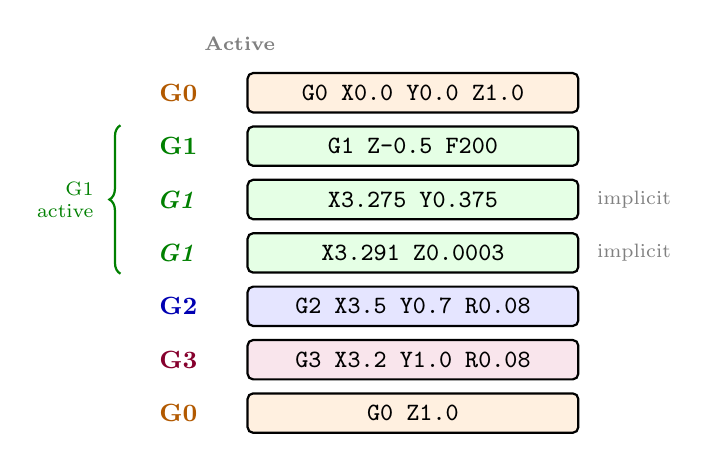
\begin{tikzpicture}[
    node distance=0.05cm,
    line/.style={rectangle, draw, thick, rounded corners=2pt, minimum width=4.2cm, minimum height=0.5cm, font=\small\ttfamily, fill=#1, align=left},
    line/.default={white},
    modal/.style={font=\small\bfseries, text=#1, anchor=east},
    modal/.default={black},
]
    % Lines — shifted right to make room for brace + labels
    \node[line=orange!12] (l1) at (0.6,0) {G0 X0.0 Y0.0 Z1.0};
    \node[line=green!10, below=0.15cm of l1] (l2) {G1 Z-0.5 F200};
    \node[line=green!10, below=0.15cm of l2] (l3) {X3.275 Y0.375};
    \node[line=green!10, below=0.15cm of l3] (l4) {X3.291 Z0.0003};
    \node[line=blue!10, below=0.15cm of l4] (l5) {G2 X3.5 Y0.7 R0.08};
    \node[line=purple!10, below=0.15cm of l5] (l6) {G3 X3.2 Y1.0 R0.08};
    \node[line=orange!12, below=0.15cm of l6] (l7) {G0 Z1.0};

    % Modal state labels — more space from boxes
    \node[modal=orange!70!black, left=0.5cm of l1] {G0};
    \node[modal=green!50!black, left=0.5cm of l2] {G1};
    \node[modal=green!50!black, left=0.5cm of l3] {\textit{G1}};
    \node[modal=green!50!black, left=0.5cm of l4] {\textit{G1}};
    \node[modal=blue!70!black, left=0.5cm of l5] {G2};
    \node[modal=purple!70!black, left=0.5cm of l6] {G3};
    \node[modal=orange!70!black, left=0.5cm of l7] {G0};

    % Annotations
    \node[font=\scriptsize\color{gray}, right=0.1cm of l3] {implicit};
    \node[font=\scriptsize\color{gray}, right=0.1cm of l4] {implicit};

    % Bracket showing modal persistence — shifted left of labels
    \draw[decorate, decoration={brace, amplitude=4pt, mirror}, thick, green!50!black]
        ([xshift=-1.6cm]l2.north west) -- ([xshift=-1.6cm]l4.south west)
        node[midway, left=6pt, font=\scriptsize, text=green!50!black, align=right] {G1\\active};

    % Header
    \node[font=\scriptsize\bfseries\color{gray}, above=0.15cm of l1, xshift=-2.2cm] {Active};
\end{tikzpicture}
\caption{Modal state persistence. Lines~3--4 contain no command word; they execute under the previously active \texttt{G1}. The active modal command (shown left, italic for implicit) carries forward until a new motion command is issued.}
\label{fig:modal_state}
\end{figure}

\subsubsection{Auxiliary Commands, Postamble, and Summary}

\emph{Canned cycles} (G81--G89) provide shorthand for drilling and boring; the controller firmware expands each into a deterministic G0/G1 sequence.\footnote{Tapping cycles (G84) additionally require spindle synchronization, a firmware operation outside the G0--G3 grammar.} The \emph{postamble} returns the machine to a safe state: spindle off (M5), coolant off (M9), home (G53~G0), program end (M30). Our tokenizer handles these as literal tokens without numeric decomposition. In our dataset, the toolpath dominates program content (80--90\% of lines), with preamble (5--10\%) and postamble (2--5\%) as fixed overhead. This distribution justifies our focus on the four core motion commands rather than the full RS-274D standard.

% ============================================================================
\subsection{Formal grammar}
\label{sec:grammar}

Given the structural regularity established in Section~\ref{sec:anatomy}, we formalize toolpath lines as lexical categories, syntactic rules, and a production grammar.

\subsubsection{Lexical Categories}

Four token types partition the vocabulary:

\begin{table}[htbp]
\centering
\caption{G-Code Token Categories}
\label{tab:token_categories}
\begin{tabular}{@{}clp{3.2cm}@{}}
\toprule
\textbf{Type} & \textbf{Category} & \textbf{Examples} \\
\midrule
0 & \textsc{Special}   & \texttt{PAD}, \texttt{BOS}, \texttt{EOS} \\
1 & \textsc{Command}   & \texttt{G0}, \texttt{G1}, \texttt{G2}, \texttt{G3} \\
2 & \textsc{Parameter} & \texttt{X}, \texttt{Y}, \texttt{Z}, \texttt{F}, \texttt{R} \\
3 & \textsc{Numeric}   & \texttt{NUM\_X\_3275}, \texttt{NUM\_R\_830} \\
\bottomrule
\end{tabular}
\end{table}

We separate addresses from values as the key design choice. \texttt{X3.275} becomes two tokens: \texttt{X} (\textsc{Parameter}) encoding \emph{which axis}, and \texttt{NUM\_X\_3275} (\textsc{Numeric}) encoding \emph{how far}. The two carry different information and benefit from independent prediction.

\subsubsection{Syntactic Rules}

Toolpath syntax follows five deterministic rules:

\begin{enumerate}[leftmargin=*]
    \item \textbf{Type Transitions.} \textsc{Command}~$\to$~\textsc{Parameter}/\texttt{EOS}; \textsc{Parameter}~$\to$~\textsc{Numeric}; \textsc{Numeric}~$\to$~\textsc{Parameter}/\texttt{EOS}. Commands and numerics never appear adjacent.

    \item \textbf{Modal Group Exclusion.} At most one command from each modal group may appear per block. The motion group \{\texttt{G0}, \texttt{G1}, \texttt{G2}, \texttt{G3}\} is mutually exclusive.

    \item \textbf{Command-Parameter Association.} Each command defines which parameters are valid, required, or forbidden (Table~\ref{tab:core_commands}).

    \item \textbf{Single-Letter Rule.} Each parameter address appears at most once per block. A line cannot contain two \texttt{X} values.

    \item \textbf{Modal Persistence.} If no command is specified, the previously active modal command persists. A line containing only \texttt{X3.291 Z0.0003} executes under the last issued motion command.
\end{enumerate}

RS-274D defines several modal groups (motion: G0--G3; plane: G17--G19; distance: G90/G91; units: G20/G21; coordinate system: G54--G59); commands within a group are mutually exclusive. Only the motion group matters during toolpath generation; the rest are set once in the preamble. Rules~1--4 apply within a single block. Rule~5 introduces cross-line state; the active modal command carries over from previous blocks. We treat each line independently, passing the modal command as external context.

\subsubsection{Command-Parameter Associations and Execution Order}

Parameter associations per the RS-274D standard~\cite{rs274d} and the NIST interpreter specification~\cite{nist_ngc} are formalized in Table~\ref{tab:core_commands}. Our framework implements X, Y, Z, F, and R; additional addresses (I, J, K, S, P) can be added per controller dialect with appropriate precision settings (Table~\ref{tab:precision}). Forbidden entries ($\times$) become $-\infty$ logit masks; required entries ($\bullet$) become positive biases (Section~\ref{sec:constrained_decoding}). The standard specifies a 21-step execution order within each block~\cite{nist_ngc}, with motion (G0--G3) at step~20 and stop codes last; our grammar does not model intra-block ordering.

\subsubsection{Formal Grammar Definition}
\label{sec:formal_grammar}

We define the per-line G-code grammar as a right-linear grammar $\mathcal{G} = (\Sigma, V, S, P)$~\cite{sipser}:

\smallskip\noindent\textbf{Terminal alphabet.}
$\Sigma = \{\texttt{BOS}, \texttt{EOS}, \texttt{G0}, \texttt{G1}, \texttt{G2}, \texttt{G3}, \texttt{X}, \texttt{Y}, \texttt{Z}, \texttt{F}, \texttt{R}, \texttt{NUM}\}$

\smallskip\noindent\textbf{Nonterminals.}
$V = \{S, \mathit{Body}, \mathit{Cmd}, \mathit{Params}, \mathit{Param}, \mathit{Addr}\}$

\smallskip\noindent\textbf{Start symbol.} $S$

\smallskip\noindent\textbf{Productions.}
\begin{align*}
S &\to \texttt{BOS}\; \mathit{Body}\; \texttt{EOS} \\
\mathit{Body} &\to \mathit{Cmd}\; \mathit{Params} \mid \mathit{Params} \\
\mathit{Cmd} &\to \texttt{G0} \mid \texttt{G1} \mid \texttt{G2} \mid \texttt{G3} \\
\mathit{Params} &\to \mathit{Addr}\; \texttt{NUM}\; \mathit{Params} \mid \varepsilon \\
\mathit{Addr} &\to \texttt{X} \mid \texttt{Y} \mid \texttt{Z} \mid \texttt{F} \mid \texttt{R}
\end{align*}

\noindent Every production is right-linear (at most one nonterminal, rightmost), so $\mathcal{G}$ generates a regular language~\cite{sipser}. The $\mathit{Addr}$ production shows the five currently implemented addresses; additional addresses (I, J, K, S, P) extend $\Sigma$ without changing the grammar's regular structure. The grammar is recognized by a five-state deterministic finite automaton; its state table, transition function, soundness and completeness arguments, and cross-line modal extension appear in Appendix~\ref{sec:dfa_construction}. The constraint mask $M$ used by Section~\ref{sec:constrained_decoding} implements $\delta$ directly, with $M(q_i, t) = -\infty$ whenever $\delta(q_i, t)$ is undefined; mask lookup is $O(1)$ since $|Q| = 5$ and $|\Sigma| = 12$.

The grammar defines 19 structural terminals: 5 special (\texttt{PAD}, \texttt{BOS}, \texttt{EOS}, \texttt{UNK}, \texttt{MASK}), 4 commands (\texttt{G0}--\texttt{G3}), 5 parameters (\texttt{X}, \texttt{Y}, \texttt{Z}, \texttt{F}, \texttt{R}), and 5 auxiliary literals (\texttt{G53}, \texttt{M3}, \texttt{M5}, \texttt{M6}, \texttt{M30}). Of these, 7--9 appear in any given dataset (Table~\ref{tab:vocab_growth}); the remainder are reserved for future extensions. Numeric values are predicted by digit heads (Section~\ref{sec:decomposition}), not vocabulary entries. Generating \texttt{G2 X3.5 Y0.7 R0.08} under the type-transition FSM of Figure~\ref{fig:grammar_constraints} illustrates the constraints: after \textsc{Parameter}~\texttt{X}, only \textsc{Numeric} is valid; after the numeric token, \texttt{X} is masked (already used) and \texttt{R} is boosted (required for G2). Each constraint evaluates in $O(1)$.

% ============================================================================
\section{A Design-Space Analysis of G-Code Tokenizers}
\label{sec:design_space}

Sections~\ref{sec:anatomy}--\ref{sec:grammar} establish the structure of the language. This section analyzes the space of tokenizers around three properties any practical G-code tokenizer should provide, and shows by case analysis over the three dominant tokenizer classes (atomic, subword, digit-decomposed) that only the third class satisfies all three simultaneously. The result is not an impossibility theorem in the formal sense of CAP or FLP: the case analysis covers the classes that dominate current practice, not a formally defined space of all conceivable tokenizers, and it is constructive in that it names what each class gives up. Section~\ref{sec:empirical} verifies each cell of Table~\ref{tab:design_space} empirically.

\subsection{Three properties}
\label{sec:three_properties}

Each definition below isolates one failure mode of standard tokenization and is stated in a testable form, so that Section~\ref{sec:empirical} can populate it with a measurement.

\begin{Definition}[Bounded vocabulary]
\label{def:bounded}
A tokenizer $T$ has \emph{bounded vocabulary} if there exists a constant $K$, independent of geometry, such that for every G-code corpus $\mathcal{C}$ at fixed precision $p$,
\[
    |V_T(\mathcal{C})| \;\le\; K,
\]
where $V_T(\mathcal{C})$ denotes the set of distinct token types $T$ emits on $\mathcal{C}$.
\end{Definition}

\begin{Definition}[Lossless coordinates]
\label{def:lossless}
A tokenizer $T$ is \emph{lossless on coordinates} if for every numeric value $v$ at supported precision $p$, the encode--decode roundtrip is exact:
\[
    \mathrm{dec}_T(\mathrm{enc}_T(v)) \;=\; v,
\]
equivalently $\sup_{v}\, |\mathrm{dec}_T(\mathrm{enc}_T(v)) - v| = 0$.
\end{Definition}

\begin{Definition}[Grammar validity]
\label{def:grammar_valid}
A tokenizer $T$ \emph{supports grammar validity} if both of the following hold:
\begin{enumerate}[leftmargin=*, label=(\roman*)]
    \item every line $\ell \in L(\mathcal{G})$ admits an unambiguous encoding $\mathrm{enc}_T(\ell) \in V_T^{\ast}$;
    \item the per-step output distribution under $T$ can be restricted---via logit masking or an equivalent constraint mechanism---to the set $L(\mathcal{G})$ without removing any line in $L(\mathcal{G})$.
\end{enumerate}
\end{Definition}

A tokenizer that maps every coordinate to a single $\langle\mathrm{NUM}\rangle$ token (e.g.\ xVal~\cite{xval}) admits encodings but fails property~(ii): the value-level distribution cannot be grammar-constrained, because the constraint mechanism has no token at which to apply the mask. Subword tokenizers fail property~(i): the same numeric value may decompose differently in different contexts, so the encoding is not unambiguous at the value level.

\subsection{A structural characterization}
\label{sec:impossibility}

We now argue, by case over the three dominant tokenizer classes, that only one of them admits all three properties of Section~\ref{sec:three_properties} simultaneously.

\begin{Proposition}[Tokenizer trichotomy over dominant classes]
\label{prop:trichotomy}
Let $T$ be a tokenizer for G-code coordinates at fixed precision $p$ over an unbounded geometric domain, drawn from one of the three standard classes: atomic (one token per coordinate value), subword (BPE- or WordPiece-style merges over the coordinate string), or digit-decomposed (each value emitted as an address letter followed by a fixed-length digit sequence). Among these three classes, only digit-decomposed tokenizers with a finite sub-vocabulary closed under composition (e.g., decimal digits with sign) satisfy Definitions~\ref{def:bounded}, \ref{def:lossless}, and~\ref{def:grammar_valid} simultaneously.
\end{Proposition}

\begin{proof}[Case analysis]
We argue by case over the three named classes of $T$. For each failing class we name the definition it violates and the structural reason.

\smallskip\noindent\textit{Case 1: atomic tokenization.} Suppose $T$ treats each coordinate as a single token. The set of quantized coordinate values at precision $p$ over an unbounded domain is countably infinite, so $T$ must either collapse infinitely many values onto finitely many tokens (violating Definition~\ref{def:lossless}) or preserve every value atomically and let $|V_T|$ scale with the observed geometric range (violating Definition~\ref{def:bounded}). Either branch fails.

\smallskip\noindent\textit{Case 2: subword tokenization.} BPE and WordPiece fragment numeric strings into merge-derived subword pieces. The fragmentation has two distinct failure modes that we separate empirically in Section~\ref{sec:exp_c}. \emph{Sub-case~2a (decode-side reinsertion):} standard HuggingFace BPE pipelines use a whitespace pre-tokenizer whose inverse inserts whitespace between pieces on decode, so an in-vocabulary value like $\texttt{0.1755}$ decodes to \texttt{"0 . 1755"} and is no longer parseable as a G-code word. This fails Definition~\ref{def:grammar_valid} property~(i) immediately, and empirically reaches $0.00 \pm 0.00\%$ free-generation grammar validity (Table~\ref{tab:exp_c}). \emph{Sub-case~2b (value-level constraint boundary):} even with a byte-level decoder that preserves the contiguous numeric string, the merge table is data-driven and context-dependent; identical values may decompose differently across contexts, and there is no consistent token slot that corresponds to a single coordinate value. This leaves Definition~\ref{def:grammar_valid} property~(ii) unsatisfied at the value level: the constraint mechanism has no semantically meaningful slot at which to enforce per-value rules (e.g., ``if this is an arc parameter, mask values outside $[0, R_{\max}]$''). Subword tokenization can be made to pass property~(i) by switching the decoder configuration, as the byte-level BPE row of Table~\ref{tab:exp_c} demonstrates, but it does not pass Definition~\ref{def:bounded} (active vocabulary grows with geometry) or the value-level form of property~(ii) simultaneously.

\smallskip\noindent\textit{Case 3: structured decomposition.} Among the three classes, only digit decomposition encodes each value as a finite alphabet that composes back to any value at precision $p$. The smallest such alphabet is the set of decimal digits together with a sign symbol, an 11-element sub-vocabulary closed under composition. Definition~\ref{def:bounded} holds because the alphabet is constant in $|\mathcal{C}|$. Definition~\ref{def:lossless} holds because digit composition is exact at precision $p$. Definition~\ref{def:grammar_valid} holds because each digit position is itself a discrete prediction slot that admits per-position masking.
\end{proof}

\paragraph{Scope of the case analysis.}
Proposition~\ref{prop:trichotomy} covers the three classes that dominate current NLP practice, treating character-level tokenization as a degenerate sub-case of decomposition over the ASCII alphabet (evaluated empirically in Section~\ref{sec:empirical}). It does not cover every conceivable tokenizer design: learned discrete codebooks, hash-based tokenization, and continuous scalar heads~\cite{xval} each require a separate argument, addressed in the remarks below. The claim is therefore a characterization over the standard families, not a universal impossibility result. In particular, the byte-level BPE result of Section~\ref{sec:exp_c} does not weaken the proposition: it shows that the subword class can satisfy property~(i) under a changed decoder configuration, while the surviving discriminators are Definition~\ref{def:bounded} (active vocabulary still grows with geometry) and the value-level form of property~(ii), which the fused-merge analysis of Proposition~\ref{prop:fused_subword} shows subword tokenizers fail regardless of decoder.

\begin{Proposition}[Fused-subword corollary]
\label{prop:fused_subword}
Let $T$ be a subword tokenizer whose learned merge table produces at least one token whose surface form fuses an address letter with one or more numeric digits (e.g., a single token spanning \texttt{X3}, \texttt{Y0}, or \texttt{R0}). Then $T$ does not admit a consistent token-position slot at which a per-value constraint mask can be applied, and therefore fails Definition~\ref{def:grammar_valid} property~(ii) at the value level, regardless of whether its decoder preserves numeric contiguity.
\end{Proposition}

\begin{proof}[Proof sketch]
A per-value constraint mask (e.g., ``if this is an arc radius, mask values outside $[R_{\min}, R_{\max}]$'') must be evaluated at a position where the decoder is choosing a coordinate value, conditioned on already having committed to an address. Fused address--digit tokens collapse the address commitment and (part of) the value into a single token choice, so the mask would have to condition on the identity of the token currently being chosen rather than on a previously emitted address; value-level constraints in standard grammar-constrained decoding frameworks do not operate this way~\cite{outlines,xgrammar,picard}. A consistent slot would require either (a) refusing to learn any fused address--digit merge, which is not a property enforced by BPE or WordPiece training, or (b) post-hoc splitting the merge at inference, which requires tokenizer-specific logic and breaks the $O(1)$ mask-lookup property. The byte-level BPE row of Table~\ref{tab:exp_c} empirically produces fused merges of this form (Table~\ref{tab:bpe_failure} shows \texttt{X3}, \texttt{Y0}, \texttt{R0}), so even though it passes property~(i), it fails property~(ii) at the value level.
\end{proof}

Proposition~\ref{prop:fused_subword} formalizes what the byte-level BPE result empirically shows: the grammar-validity gap between BPE configurations is a property-(i) issue solved by the decoder configuration, but the grammar-\emph{constrainability} gap between BPE and digit decomposition is a property-(ii) issue that survives any decoder configuration, because the underlying merge table has already collapsed the address--value boundary.

\paragraph{Remarks on the case analysis.}
Three variations leave the characterization unchanged. \textit{Variable per-parameter precision} (Table~\ref{tab:precision}) does not change the argument: each address $a$ gets its own digit-position count $n_a$, the operative alphabet is still the eleven decimal digits plus sign, and the decomposed sub-vocabulary remains constant in $|\mathcal{C}|$. \textit{Mixed atomic-and-decomposed hybrids} inherit the worst failure of each component: any atomically encoded address still has unbounded geometric range and fails Definition~\ref{def:bounded}. \textit{Structured tokenizers with reserved literals} (such as ours, which adds 19 fixed literals to an 11-element digit alphabet) preserve Definition~\ref{def:bounded} because the literals are constant in $|\mathcal{C}|$.

Two structural classes lie outside the three named classes of Proposition~\ref{prop:trichotomy}. \emph{Continuous-valued tokenizers} such as xVal~\cite{xval} replace the value-level token with a scalar head; Definition~\ref{def:grammar_valid} property~(ii) fails by inspection because the constraint mechanism has no discrete token slot at which to apply a value-level mask. \emph{Learned discrete codebooks} (e.g., VQ-style value quantizers) can in principle occupy the all-checkmarks corner if the codebook is closed under composition, but we do not evaluate them in this work. The unquantized limit $p \to 0$ has an uncountable value space, so Definition~\ref{def:bounded} fails for every token-based tokenizer; our reliance on a fixed positive $p$ is a necessary precondition for the all-checkmarks corner to exist at all.

Proposition~\ref{prop:trichotomy} thus locates the framework's design choices within current tokenizer practice: among the three classes standard NLP systems use, digit decomposition alone occupies the (\textsc{Bounded}, \textsc{Lossless}, \textsc{Grammar}) corner, and the grammar-constrained decoding of Section~\ref{sec:constrained_decoding} activates property~(ii) of Definition~\ref{def:grammar_valid}.

Experiment~C (Section~\ref{sec:exp_c}) measures the two sub-failures of Case~2 separately: the standard whitespace-pre-tokenized BPE rows exhibit sub-case~2a, and a byte-level BPE control isolates the merge-table ambiguity of sub-case~2b from the decoder configuration.

\subsection{Worked example: tokenizing R0.1755}
\label{sec:worked_example}

To make the trichotomy of Proposition~\ref{prop:trichotomy} concrete, we trace what each of the three structural cases does on a single G-code parameter, the arc-radius value \texttt{R0.1755}. We pick \texttt{R} (rather than \texttt{X} or \texttt{Y}) so that the underlying value is exactly representable at the supported precision: in our implementation \texttt{R} uses precision $p = 0.0001\,$in (Table~\ref{tab:precision}), so $0.1755$ quantizes to bucket $1755$ without rounding error. Each row of Table~\ref{tab:worked_example} represents one tokenizer occupying one of the three structural cases, encodes \texttt{R0.1755}, and reports which definitions it satisfies.

\begin{table}[htbp]
\centering
\caption{Worked Example: \texttt{R0.1755} Through One Tokenizer per Structural Case}
\label{tab:worked_example}
\small
\begin{tabular}{@{}p{2.6cm}p{4.4cm}cccp{3.0cm}@{}}
\toprule
\textbf{Tokenizer} & \textbf{Encoded form} & \textbf{Def.~\ref{def:bounded}} & \textbf{Def.~\ref{def:lossless}} & \textbf{Def.~\ref{def:grammar_valid}} & \textbf{Failure mode} \\
\midrule
\textbf{Case 1: Atomic} \newline Flat per-value &
\texttt{[R0.1755]} (1 token) &
$\times$ & $\checkmark$ & $\checkmark$ &
Vocabulary scales with geometry: every new arc radius adds a new token; held-out OOV reaches 18--65\% (Table~\ref{tab:exp_d_oov}). \\
\addlinespace
\textbf{Case 2: Subword} \newline Domain BPE &
\texttt{[R, 0, ., 17, 55]} (5 tokens) &
$\checkmark$ & $\sim$ & $\times$ &
Decoder reinserts whitespace at every BPE boundary, producing \texttt{"R0 . 1755"}; the parser cannot recover the address--value pair, even though every subword is correct. \\
\addlinespace
\textbf{Case 3: Decomposed} \newline Hierarchical (ours) &
\texttt{[R, SIGN+, D1, D7, D5, D5]} (6 tokens) &
$\checkmark$ & $\checkmark$ & $\checkmark$ &
None: the address letter \texttt{R}, sign, and four digit positions compose back to the integer bucket $1755$, which decodes to the value $1755 \times 0.0001 = 0.1755\,$in exactly, and each prediction slot admits per-position grammar masking. \\
\bottomrule
\end{tabular}
\end{table}

All three rows encode the same physical quantity. The differences are not in what the tokenizer can in principle represent but in which definition each one structurally fails: Case 1 makes vocabulary unbounded, Case 2 makes the value-to-string round trip ambiguous, and Case 3 is the only configuration in which all three definitions hold simultaneously.

The Case~2 row fails by the decode-time mechanism of sub-case~2a: the five subword pieces \texttt{[R, 0, ., 17, 55]} are individually correct, and a trained decoder under this tokenizer routinely predicts the right subword sequence in our experiments (Section~\ref{sec:exp_c}), but the whitespace-reinserting decode reassembles them as \texttt{"R0 . 1755"}, which the regex-based G-code parser cannot recognize as a parameter--value pair. This is property~(i) of Definition~\ref{def:grammar_valid} failing in practice, and it explains the $0.00 \pm 0.00\%$ free-generation grammar validity reported for every BPE row of Table~\ref{tab:exp_c} across five folds and 552 test samples. The exact fragmentation is value-dependent: for radii such as \texttt{R0.083} the same merge table instead fuses the address letter into an \texttt{R0} token (Table~\ref{tab:bpe_failure}), the fused address--value merge that Proposition~\ref{prop:fused_subword} shows blocks value-level constraints regardless of the decoder.

The exact representability is specific to \texttt{R}: coarser-precision parameters (\texttt{X}, \texttt{Y}, \texttt{Z} at $p = 0.001\,$in; Table~\ref{tab:precision}) would incur a quantization error bounded by $p/2$ on the same value. Experiment~B confirms this empirically: the mean reconstruction error on \texttt{X}, \texttt{Y}, and \texttt{Z} is approximately $0.00025\,$in ($6.4\,\mu$m), within the $p/2 = 0.0005\,$in bound.

\subsection{Tokenizer families and the design space}
\label{sec:tokenizer_families}

Table~\ref{tab:design_space} maps the tokenizer families onto the three axes. Each entry is verified empirically in Section~\ref{sec:empirical}: vocabulary growth (Experiment~A) populates the \textsc{Bounded} column, coordinate reconstruction error (Experiment~B) populates the \textsc{Lossless} column, free-generation grammar validity (Experiment~C) populates the \textsc{Grammar} column, and held-out OOV rate (Experiment~D) confirms that vocabulary boundedness is a measurable failure mode rather than a definitional artifact.

\begin{table}[htbp]
\centering
\caption{Design-Space Coverage of G-Code Tokenizer Families}
\label{tab:design_space}
\scriptsize
\begin{tabular}{@{}lccc@{}}
\toprule
\textbf{Tokenizer family} & \textbf{Bounded $V$} & \textbf{Lossless} & \textbf{Grammar} \\
\midrule
GPT-4 BPE (cl100k)            & $\checkmark$ & $\times$ & $\sim^{\ast\ast}$ \\
GPT-2 BPE (r50k)              & $\checkmark$ & $\times$ & $\sim^{\ast\ast}$ \\
Domain BPE (whitespace)       & $\checkmark$ & $\times$ & $\times^{\ast}$ \\
Domain BPE (byte-level)       & $\checkmark$ & $\times$ & $\sim^{\ast\ast}$ \\
WordPiece                     & $\checkmark$ & $\times$ & $\times^{\ast}$ \\
Flat per-value                & $\times$     & $\checkmark$ & $\checkmark$ \\
Character-level               & $\checkmark$ & $\checkmark$ & $\times^{\ast{\ast}\ast}$ \\
xVal scalar~\cite{xval}$^{\#}$       & $\checkmark$ & $\sim^{\dagger}$ & $\times$ \\
Regression head$^{\#}$               & $\checkmark$ & $\sim^{\dagger}$ & $\sim^{\ddagger}$ \\
\midrule
\textbf{Hierarchical + digits (ours)} & $\boldsymbol{\checkmark}$ & $\boldsymbol{\checkmark}$ & $\boldsymbol{\checkmark}$ \\
\bottomrule
\multicolumn{4}{@{}p{6.3cm}}{\scriptsize $^{\ast}$Fails Def.~\ref{def:grammar_valid} via sub-case~2a (decoder-side whitespace reinsertion); empirical grammar validity $0.00\pm0.00\%$ (Table~\ref{tab:exp_c}).}\\
\multicolumn{4}{@{}p{6.3cm}}{\scriptsize $^{\ast\ast}$Passes property~(i) when the decode path preserves numeric contiguity (byte-level BPE empirically at $97\%$; GPT-4 compact at $97\%$), but still fails the value-level form of property~(ii) because the merge table exposes no consistent token boundary for address--value pairs.}\\
\multicolumn{4}{@{}p{6.3cm}}{\scriptsize $^{\ast{\ast}\ast}$Char-level FSAs over digit strings explode combinatorially before grammar productions can attach.}\\
\multicolumn{4}{@{}p{6.3cm}}{\scriptsize $^{\dagger}$Bounded by float precision, not exact at quantized precision $p$.}\\
\multicolumn{4}{@{}p{6.3cm}}{\scriptsize $^{\ddagger}$Constrainable at the address level but not at the value level.}\\
\multicolumn{4}{@{}p{6.3cm}}{\scriptsize $^{\#}$Theoretical placement based on published behavior; not evaluated empirically in this work. The other rows are trained and measured on our 120-file corpus (Section~\ref{sec:empirical}).}
\end{tabular}
\normalsize
\end{table}

The remainder of the paper presents the constructive instantiation of the bottom row and the empirical support for the rest.

Figure~\ref{fig:design_space_cube} renders Table~\ref{tab:design_space} as a three-axis cube. Each corner is a $(\textsc{Bounded}, \textsc{Lossless}, \textsc{Grammar})$ Boolean tuple, and each tokenizer family lives at the corner that matches its row in the table. Five of the eight corners are occupied; three are empty (e.g.\ $(\textsc{Bounded},\textsc{Lossless},\neg\textsc{Grammar})$ in our taxonomy contains only character-level, and $(\neg\textsc{Bounded},\neg\textsc{Lossless},\textsc{Grammar})$ is structurally empty under our definitions). Proposition~\ref{prop:trichotomy} is the statement that exactly one corner, $(\textsc{Bounded},\textsc{Lossless},\textsc{Grammar})$, contains the hierarchical decomposition family and that every other tokenizer architecture must accept at least one $\neg$ in its tuple.

\begin{figure}[htbp]
\centering
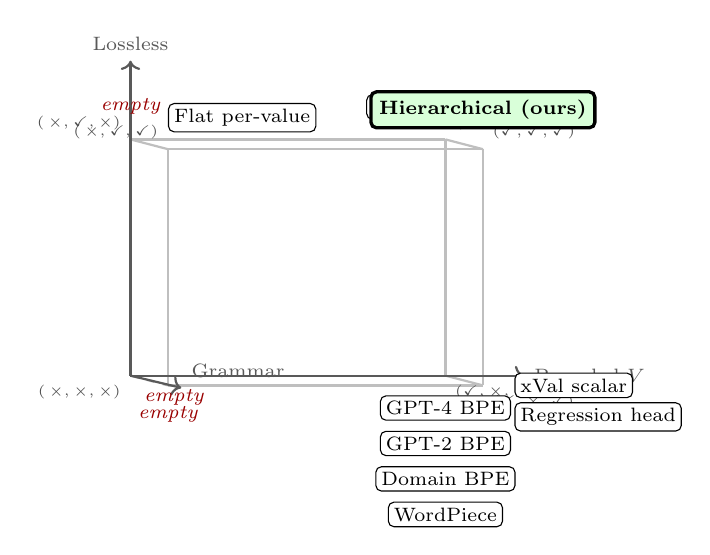
\begin{tikzpicture}[
    every node/.style={font=\scriptsize},
    axis/.style={->, thick, gray!70!black},
    cube/.style={thick, gray!50},
    tok/.style={draw, fill=white, rounded corners=2pt, inner sep=2pt, font=\scriptsize},
    ours/.style={draw, very thick, fill=green!15, rounded corners=2pt, inner sep=3pt, font=\scriptsize\bfseries},
    none/.style={font=\scriptsize\itshape\color{red!60!black}},
]
% Cube vertices: each is a (B, L, G) corner.
% B (Bounded) along x; L (Lossless) along y; G (Grammar) along z.
% origin = (0,0,0) = (-, -, -)
\coordinate (mmm) at (0,0,0);
\coordinate (Bmm) at (4,0,0);
\coordinate (mLm) at (0,3,0);
\coordinate (BLm) at (4,3,0);
\coordinate (mmG) at (1.4,0.8,2.4);
\coordinate (BmG) at (5.4,0.8,2.4);
\coordinate (mLG) at (1.4,3.8,2.4);
\coordinate (BLG) at (5.4,3.8,2.4);

% Cube edges (back / hidden first, then front)
\draw[cube, dashed] (mmm) -- (Bmm);
\draw[cube, dashed] (mmm) -- (mLm);
\draw[cube, dashed] (mmm) -- (mmG);
\draw[cube] (Bmm) -- (BLm);
\draw[cube] (mLm) -- (BLm);
\draw[cube] (Bmm) -- (BmG);
\draw[cube] (mLm) -- (mLG);
\draw[cube] (mmG) -- (BmG);
\draw[cube] (mmG) -- (mLG);
\draw[cube] (BmG) -- (BLG);
\draw[cube] (mLG) -- (BLG);
\draw[cube] (BLm) -- (BLG);

% Axes
\draw[axis] (mmm) -- ++(5.0,0,0) node[right, font=\scriptsize] {Bounded $V$};
\draw[axis] (mmm) -- ++(0,4.0,0) node[above, font=\scriptsize] {Lossless};
\draw[axis] (mmm) -- ++(1.8,1.0,3.0) node[above right, font=\scriptsize] {Grammar};

% Corner labels (Boolean tuples in subscript form)
\node[font=\tiny\color{gray!60!black}, below left] at (mmm) {$(\,\times,\times,\times)$};
\node[font=\tiny\color{gray!60!black}, below right] at (Bmm) {$(\checkmark,\times,\times)$};
\node[font=\tiny\color{gray!60!black}, above left] at (mLm) {$(\,\times,\checkmark,\times)$};
\node[font=\tiny\color{gray!60!black}, above right] at (BLm) {$(\checkmark,\checkmark,\times)$};
\node[font=\tiny\color{gray!60!black}, below right] at (BmG) {$(\checkmark,\times,\checkmark)$};
\node[font=\tiny\color{gray!60!black}, above left] at (mLG) {$(\,\times,\checkmark,\checkmark)$};
\node[font=\tiny\color{gray!60!black}, above right] at (BLG) {$(\checkmark,\checkmark,\checkmark)$};

% Tokenizer family labels at each occupied corner
\node[tok, anchor=north] at ($(Bmm) + (0, -0.25)$) {GPT-4 BPE};
\node[tok, anchor=north] at ($(Bmm) + (0, -0.7)$) {GPT-2 BPE};
\node[tok, anchor=north] at ($(Bmm) + (0, -1.15)$) {Domain BPE};
\node[tok, anchor=north] at ($(Bmm) + (0, -1.6)$) {WordPiece};

\node[tok, anchor=west] at ($(mLG) + (-0.0, 0.4)$) {Flat per-value};

\node[tok, anchor=south] at ($(BLm) + (0.0, 0.25)$) {Character-level};

\node[tok, anchor=west] at ($(BmG) + (0.4, 0.0)$) {xVal scalar};
\node[tok, anchor=west] at ($(BmG) + (0.4, -0.4)$) {Regression head};

\node[ours] at ($(BLG) + (0.0, 0.5)$) {Hierarchical (ours)};

% Empty corners
\node[none, anchor=north west] at ($(mmm) + (0.05, -0.05)$) {empty};
\node[none, anchor=south] at ($(mLm) + (0, 0.2)$) {empty};
\node[none, anchor=north] at ($(mmG) + (0, -0.15)$) {empty};
\end{tikzpicture}
\caption{The (\textsc{Bounded}, \textsc{Lossless}, \textsc{Grammar}) design space as a three-axis Boolean cube. Each axis is one of the three properties of Definitions~\ref{def:bounded}--\ref{def:grammar_valid}; each corner is a possible combination; each tokenizer family lives at the corner whose Boolean tuple matches its row in Table~\ref{tab:design_space}. Proposition~\ref{prop:trichotomy} is the statement that the front-top-right corner $(\checkmark,\checkmark,\checkmark)$ is reachable only by the structured-decomposition family (Case~3 of the proof), and the dashed cube edges denote unreachable transitions: no incremental modification of an atomic or subword tokenizer can move it into the all-checkmarks corner without changing its structural class.}
\label{fig:design_space_cube}
\end{figure}

% ============================================================================
\section{Method}
\label{sec:method}

The method instantiates the digit-decomposition corner of Table~\ref{tab:design_space} in three parts: canonicalization and hybrid tokenization (Section~\ref{sec:tokenization}), the hierarchical token decomposition that occupies Case~3 of Proposition~\ref{prop:trichotomy} (Section~\ref{sec:decomposition}), and the grammar-constrained decoding mechanism that activates property~(ii) of Definition~\ref{def:grammar_valid} (Section~\ref{sec:constrained_decoding}).

\subsection{Tokenization scheme}
\label{sec:tokenization}

\subsubsection{Canonicalization}

Raw G-code undergoes five normalization steps to eliminate surface variation across CAM systems: (1)~strip comments (\texttt{;} and \texttt{(...)}), (2)~strip line numbers (\texttt{N}-codes) and checksums, (3)~uppercase, (4)~normalize leading zeros on command codes (\texttt{G01}~$\to$~\texttt{G1}), and (5)~collapse whitespace.

\noindent For example, \texttt{n20 g02 x3.275 r0.083 ; arc} canonicalizes to \texttt{G2 X3.275 R0.083}.

\paragraph{Variable-precision coordinate strings.}
Step~4 is the only normalization step that touches numeric values, and it applies only to command leading zeros. Trailing-zero differences on coordinate strings (\texttt{X3.2} vs.\ \texttt{X3.2000}) are \emph{not} resolved at canonicalization. Quantization (below) makes them equivalent by mapping both to the same integer bucket at the parameter's precision, in this case $\text{round}(3.2 / 0.001) = \text{round}(3.2000 / 0.001) = 3200$, emitted as \texttt{NUM\_X\_3200}. The tokenizer is therefore firmware-agnostic. TinyG (the controller on our Bantam Tools desktop CNC mill), grbl, and other firmwares that interpret trailing zeros differently in their parsers all receive identical tokens from our preprocessing, because bucket-level quantization absorbs the distinction before the model sees any coordinate.

\subsubsection{Hybrid Tokenization}

We use a \emph{hybrid} strategy. Literal mode creates one token per coordinate value (vocabulary explosion). Split mode over-fragments commands (\texttt{G1} $\to$ \texttt{G}, \texttt{1}). Hybrid mode preserves command semantics while separating addresses from values:

\begin{lstlisting}
G2 X3.275 Y0.375 R0.083
-> [BOS, G2, X, NUM_X_3275, Y,
    NUM_Y_375, R, NUM_R_830, EOS]
\end{lstlisting}

\subsubsection{Quantization}

We quantize numeric values at domain-appropriate precision, mapping a float value $v$ for parameter $a$ to an integer bucket:
\begin{equation}
    \text{bucket}(v, a) = \text{round}\!\left(\frac{v}{\text{precision}(a)}\right)
\end{equation}

\noindent For example, \texttt{X3.275} $\to$ $\text{round}(3.275/0.001) = 3275$ $\to$ \texttt{NUM\_X\_3275}; \texttt{R0.083} $\to$ $\text{round}(0.083/0.0001) = 830$ $\to$ \texttt{NUM\_R\_830}.

Table~\ref{tab:precision} combines quantization precision, value ranges, and digit-head configuration for each parameter.

\begin{table}[htbp]
\centering
\caption{Parameter Precision, Ranges, and Digit Configuration. Linear values are in inches; the corpus G-code runs in \texttt{G20} (inch) mode. The Range column is the implementation's native-unit validation clamp, not the machine envelope.}
\label{tab:precision}
\small
\begin{tabular}{@{}lllcc@{}}
\toprule
\textbf{Param} & \textbf{Prec.} & \textbf{Range} & \textbf{Int.} & \textbf{Dec.} \\
\midrule
X, Y  & 0.001\,in  & $\pm$500\,in     & 2 & 4 \\
Z     & 0.001\,in  & $-$200--50\,in   & 1 & 4 \\
I, J  & 0.0001\,in & $\pm$500\,in     & 1 & 4 \\
R     & 0.0001\,in & 0.001--500\,in   & 1 & 4 \\
F     & 1\,in/min  & 0.1--15000       & 2 & 1 \\
S     & 10\,RPM    & 0--30000         & 5 & 0 \\
\bottomrule
\end{tabular}
\normalsize

\smallskip
{\small Int.\ = max integer digits, Dec.\ = decimal digits. These define digit-head dimensionality per parameter.}
\end{table}

\subsubsection{The Vocabulary Explosion Problem}

Table~\ref{tab:vocab_comparison} quantifies the problem for a single workpiece. Each new part compounds OOV failures.

\begin{table}[htbp]
\centering
\caption{Vocabulary Size vs.\ Precision}
\label{tab:vocab_comparison}
\begin{tabular}{@{}lccr@{}}
\toprule
\textbf{Strategy} & \textbf{Size} & \textbf{OOV} & \textbf{\% Numeric} \\
\midrule
2-digit bucketed   & 170  & $\sim$0\%  & 87\% \\
Full precision     & 712  & 0\%        & 97.3\% \\
Digit-by-digit     & 19   & 0\%        & 0\%$^\dagger$ \\
\bottomrule
\multicolumn{4}{l}{\footnotesize $^\dagger$Numeric values predicted by digit heads, not vocabulary.}
\end{tabular}
\end{table}

Figure~\ref{fig:vocab_scaling} plots measured vocabulary growth across our 120-file dataset (Section~\ref{sec:empirical}). Flat vocabulary reaches 4{,}435 tokens while structural vocabulary stays at 9 (19-slot capacity).

% Vocab explosion figure — measured from 120-file dataset
\begin{figure}[htbp]
\centering
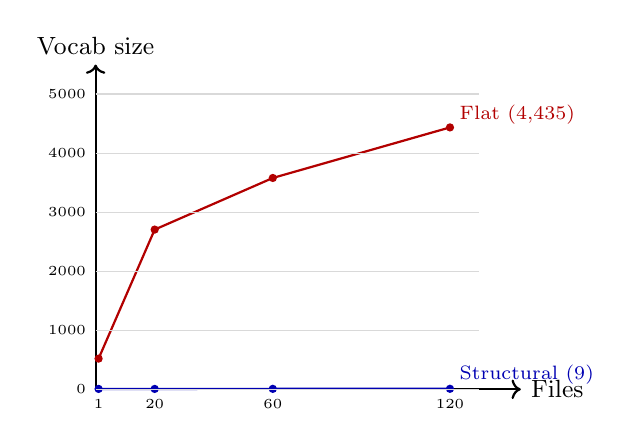
\begin{tikzpicture}[scale=0.75]
    \begin{scope}
    % Axes
    \draw[->, thick] (0,0) -- (7.2,0) node[right, font=\small] {Files};
    \draw[->, thick] (0,0) -- (0,5.5) node[above, font=\small] {Vocab size};

    % Scale: x = files/20, y = tokens/1000
    % Data (flat vocab incl. structural, matches Table tab:vocab_growth / growth.csv):
    % 1->520, 20->2705, 60->3579, 120->4435

    % Flat vocab (measured)
    \draw[thick, red!70!black] plot coordinates {
        (0.05, 0.520) (1.0, 2.705) (3.0, 3.579) (6.0, 4.435)
    };
    \fill[red!70!black] (0.05, 0.520) circle (2pt);
    \fill[red!70!black] (1.0, 2.705) circle (2pt);
    \fill[red!70!black] (3.0, 3.579) circle (2pt);
    \fill[red!70!black] (6.0, 4.435) circle (2pt);
    \node[font=\scriptsize, red!70!black, right] at (6.0, 4.65) {Flat (4{,}435)};

    % Structural vocab (measured, essentially flat)
    \draw[thick, blue!70!black] plot coordinates {
        (0.05, 0.007) (1.0, 0.007) (3.0, 0.008) (6.0, 0.009)
    };
    \fill[blue!70!black] (0.05, 0.007) circle (2pt);
    \fill[blue!70!black] (1.0, 0.007) circle (2pt);
    \fill[blue!70!black] (3.0, 0.008) circle (2pt);
    \fill[blue!70!black] (6.0, 0.009) circle (2pt);
    \node[font=\scriptsize, blue!70!black, right] at (6.0, 0.25) {Structural (9)};

    % Y-axis labels
    \foreach \y/\l in {0/0, 1/1000, 2/2000, 3/3000, 4/4000, 5/5000} {
        \node[font=\tiny, left] at (0, \y) {\l};
        \draw[gray!30] (0, \y) -- (6.5, \y);
    }

    % X-axis labels
    \foreach \x/\l in {0.05/1, 1.0/20, 3.0/60, 6.0/120} {
        \node[font=\tiny, below] at (\x, 0) {\l};
    }
    \end{scope}
\end{tikzpicture}
\caption{Measured vocabulary growth across 120 G-code files. Flat vocabulary grows from 520 to 4{,}435 tokens; structural vocabulary remains fixed at 7--9 tokens. The numeric fraction rises from 97.3\% (single part, Table~\ref{tab:vocab_comparison}) to 99.8\% across 120 files. Data from Table~\ref{tab:vocab_growth}.}
\label{fig:vocab_scaling}
\end{figure}

\subsubsection{End-to-End Pipeline}

Figure~\ref{fig:pipeline} (Appendix~\ref{sec:appendix}) traces a single G-code line through the complete pipeline: canonicalization, hybrid tokenization, type classification, hierarchical decomposition, and digit-by-digit prediction.

% ============================================================================
\subsection{Hierarchical token decomposition}
\label{sec:decomposition}

% Decoder architecture overview
\subsubsection{From Flat to Structured Prediction}

A flat vocabulary selects from $|\mathcal{V}|$ classes with no structural bias; the model must independently learn that \texttt{NUM\_X\_3275} and \texttt{NUM\_X\_3276} are numerically adjacent. Our hierarchical approach decomposes prediction into a cascade:
\begin{equation}
    P(\text{token}) = P(\tau) \cdot P(\iota \mid \tau) \cdot P(\mathbf{v} \mid \iota, \tau)
\end{equation}
where $\tau$ is the token type, $\iota$ is the identity (command or parameter address), and $\mathbf{v}$ is the numeric value. This factorization follows the class-based language model tradition~\cite{brown_classlm,morin_hsoftmax}, in which tokens are grouped into classes (types) and prediction proceeds hierarchically through class then member. Our contribution is not the factorization itself but its instantiation for G-code. The classes are grammar-derived rather than learned, the third level decomposes into digits rather than selecting from a fixed set, and the entire cascade integrates with the DFA-based grammar constraints from Section~\ref{sec:formal_grammar}. Figure~\ref{fig:decomposition_detail} (Appendix~\ref{sec:appendix}) illustrates this cascade with a concrete example.

\subsubsection{Level 1: Token Type (4 classes)}

A four-way classifier determines the token's role, the ``part of speech'' of G-code. This prediction is nearly deterministic given the grammar; after \textsc{Parameter}, the type \emph{must} be \textsc{Numeric}.

\subsubsection{Level 2: Identity Prediction}

Conditioned on token type:
\begin{itemize}[leftmargin=*]
    \item \textsc{Command} $\to$ \{G0, G1, G2, G3\} (4 classes)
    \item \textsc{Parameter} $\to$ \{X, Y, Z, F, R, ...\} (5+ classes)
    \item \textsc{Special} $\to$ \{PAD, BOS, EOS, UNK, MASK\} (5 classes)
    \item \textsc{Numeric} $\to$ proceed to Level~3
\end{itemize}

\subsubsection{Level 3: Digit-by-Digit Numeric Prediction}

Instead of predicting a numeric token as one of hundreds of vocabulary entries, we decompose each value into structured components:

\begin{equation}
    v = s \cdot \left( \sum_{i=0}^{1} d_i \cdot 10^{1-i} + \sum_{j=0}^{3} d_{2+j} \cdot 10^{-(j+1)} \right)
\end{equation}

where $s \in \{+1, -1, 0\}$ is the sign and $d_0, \ldots, d_5 \in \{0, \ldots, 9\}$ are the six digits in the format $\pm d_0 d_1 . d_2 d_3 d_4 d_5$.

\begin{table}[htbp]
\centering
\caption{Digit-by-Digit Decomposition Examples}
\label{tab:digit_examples}
\small
\begin{tabular}{@{}lrllc@{}}
\toprule
\textbf{Token} & \textbf{Val.} & \textbf{Sign} & \textbf{Digits} & \textbf{Format} \\
\midrule
\texttt{NUM\_X\_3291}  & 3.291  & $+$ & $[0,3,2,9,1,0]$ & $+03.2910$ \\
\texttt{NUM\_Y\_375}   & 0.375  & $+$ & $[0,0,3,7,5,0]$ & $+00.3750$ \\
\texttt{NUM\_Z\_n43}   & $-$0.043 & $-$ & $[0,0,0,4,3,0]$ & $-00.0430$ \\
\texttt{NUM\_R\_830}   & 0.083  & $+$ & $[0,0,0,8,3,0]$ & $+00.0830$ \\
\bottomrule
\end{tabular}
\normalsize

{\small\textit{Note:} The 6-digit format applies to positional parameters. Feed rate (F) uses fewer digits ($d_0 d_1.d_2$). The digit head is parameter-aware: each address specifies its own digit count to match its physical resolution.}
\end{table}

This decomposition provides five advantages: (1)~\textbf{zero OOV}, since any value is representable; (2)~\textbf{numeric proximity}, since 3.275 and 3.276 differ in one digit; (3)~\textbf{compositionality}, since each digit is a 10-class problem; (4)~\textbf{precision control}, since digits can be appended without vocabulary growth; and (5)~\textbf{generalization}, since the scheme works for any geometry without retraining.

\textbf{Why digits, not regression?} A regression head (like our auxiliary $\hat{v}$) produces a point estimate, losing the ability to express structured uncertainty (e.g., confident that the integer part is 3 but uncertain whether the fourth decimal is 2 or 3). Digit heads produce a joint distribution over the value space and integrate with grammar-based logit masking, which has no analogue for continuous outputs. xVal~\cite{xval} takes the regression approach, preserving magnitude but losing both digit-level structure and constraint compatibility.

\textbf{Limitation: digit independence.} The six heads predict independently. To characterize the cost of this assumption, we compute the mutual information (MI) and its normalized form (normalized mutual information, NMI) between adjacent digit positions across 13{,}595 numeric values in our dataset:

\begin{center}
\scriptsize
\begin{tabular}{@{}lcccc@{}}
\toprule
\textbf{Pair} & $d_0$-$d_1$ & $d_1$-$d_2$ & $d_2$-$d_3$ & $d_3$-$d_4$ \\
\midrule
MI (bits)  & 0.01 & 0.85 & 0.45 & 0.09 \\
NMI        & 0.86 & 0.87 & 0.17 & 0.03 \\
\bottomrule
\end{tabular}
\end{center}

\noindent The integer-decimal boundary ($d_1$-$d_2$) exhibits strong dependency (0.85 bits), as expected, since knowing the integer part constrains the decimal range. Later decimal positions ($d_3$-$d_5$) are near-independent (MI $< 0.2$ bits, NMI $< 0.06$). An autoregressive chain predicting $d_0 \to d_1 \to d_2$ then independent $d_3$-$d_5$ could capture the high-MI boundary while keeping most predictions parallel.

\subsubsection{Conditioning Signals}

Digit prediction is conditioned on the \textbf{parameter type} (X, Y, Z, F, R), which determines the physical quantity and range, and the \textbf{operation type} (face, pocket, adaptive), which influences typical value distributions. These embeddings are concatenated with the hidden state and projected before digit prediction.

\subsubsection{Training Objective}

The hierarchical decomposition yields a multi-head loss:

\begin{equation}
\mathcal{L} = \mathcal{L}_\tau + \mathcal{L}_\iota + \mathcal{L}_s + \sum_{i=0}^{5} \mathcal{L}_{d_i} + \lambda_{\text{aux}} \mathcal{L}_{\hat{v}} + \mathcal{L}_{\text{grammar}}
\label{eq:loss}
\end{equation}

where $\mathcal{L}_\tau$, $\mathcal{L}_\iota$, $\mathcal{L}_s$, $\mathcal{L}_{d_i}$ are cross-entropy losses on type (4), identity, sign (3), and digit (10) predictions; $\mathcal{L}_{\hat{v}}$ is Huber loss on an auxiliary scalar prediction ($\lambda_{\text{aux}} = 0.1$); and $\mathcal{L}_{\text{grammar}}$ sums soft constraint penalties (Section~\ref{sec:constrained_decoding}). Losses are masked to apply only at positions of the corresponding type.

\subsubsection{Token Reassembly}

Given predictions from all levels, a G-code token is reassembled deterministically:

\begin{algorithmic}[1]
\small
\Function{Reassemble}{$\tau$, $\iota$, $s$, $\mathbf{d}$}
    \If{$\tau \in \{\text{Spcl, Cmd, Par}\}$}
        \State \Return lookup$[\tau, \iota]$  \Comment{e.g.\ \texttt{G2}, \texttt{X}, \texttt{EOS}}
    \ElsIf{$\tau = \text{Num}$}
        \State $v \gets \sum_i d_i \cdot 10^{1-i}$  \Comment{compose digits}
        \State \textbf{if} $s = -$ \textbf{then} $v \gets -v$
        \State $a \gets \text{last\_param\_address}$
        \State \Return \texttt{NUM\_\{$a$\}\_\{round($v$/prec($a$))\}}
    \EndIf
\EndFunction
\end{algorithmic}

\smallskip\noindent Reassembly closes the loop: hierarchical predictions $\to$ digits $\to$ G-code token $\to$ valid line.

\paragraph{Inference-time overhead.}
The hierarchical head cascade replaces a single $d_{\text{model}} \to 712$ softmax with nine smaller projections ($d_{\text{model}} \to \{4, 14, 3\}$ plus six $d_{\text{model}} \to 10$ digit heads). On a CPU micro-benchmark ($d_{\text{model}} = 384$, single-sample forward pass, 1000-iteration mean), the flat head costs $\approx\!38\,\mu$s/token and the hierarchical cascade costs $\approx\!73\,\mu$s/token, an overhead of $+35\,\mu$s per token, roughly $+93\%$ over the flat head. In absolute terms this is still well below real-time CNC monitoring latency budgets. Even at a hypothetical 50\,Hz monitoring rate (a 20\,ms budget per window), a single token costs $\approx\!73\,\mu$s ($\sim\!270\times$ headroom) and decoding a full $7$--$9$-token line costs $\approx\!0.5$--$0.66\,$ms ($\sim\!30$--$40\times$ headroom), before adding the sensor-encoder forward pass. The overhead is dominated by kernel launch cost on small tensors; on GPU or with batched inference the relative cost shrinks because the heads can run in parallel. We therefore treat the cascade overhead as negligible for monitoring applications.

% ============================================================================
\subsection{Grammar-constrained decoding}
\label{sec:constrained_decoding}

We enforce the grammar via hard constraints (inference-time logit masking) and soft constraints (training-time penalties).

\subsubsection{Hard Constraints via Logit Masking}

The logit mask implements the DFA transition function from Section~\ref{sec:formal_grammar}. Define $M: Q \times \Sigma \to \{0, -\infty\}$ as:
\begin{equation}
    M(q, t) = \begin{cases} 0 & \text{if } \delta(q, t) \text{ is defined} \\ -\infty & \text{otherwise} \end{cases}
\end{equation}
At each decoding step, the masked logits are $\tilde{\ell}^{(t)} = \ell^{(t)} + M(q_t, \cdot)$ where $q_t$ is the current DFA state. By construction, the mask is \textbf{sound}: every generated sequence is in $L(\mathcal{A}) = L(\mathcal{G})$, since only transitions defined in $\delta$ have non-zero probability. It is also \textbf{complete}: every string in $L(\mathcal{G})$ can be generated, since the mask never blocks a valid transition.

Table~\ref{tab:type_transitions} shows the mask in tabular form.

\begin{table}[htbp]
\centering
\caption{Type Transition Mask ($\checkmark$ = valid, $\times$ = masked to $-\infty$)}
\label{tab:type_transitions}
\begin{tabular}{@{}lcccc@{}}
\toprule
\textbf{Prev.} & \textsc{Spcl} & \textsc{Cmd} & \textsc{Par} & \textsc{Num} \\
\midrule
\texttt{BOS}       & $\times$ & $\checkmark$ & $\checkmark$ & $\times$ \\
\textsc{Command}   & EOS      & $\times$ & $\checkmark$ & $\times$ \\
\textsc{Parameter} & $\times$ & $\times$ & $\times$ & $\checkmark$ \\
\textsc{Numeric}   & EOS      & $\times$ & $\checkmark$ & $\times$ \\
\bottomrule
\end{tabular}
\end{table}

Beyond type transitions, command-specific rules further constrain parameter selection:
\begin{itemize}[leftmargin=*]
    \item \textbf{G0 $\to$ no F.} Rapid traversals have no programmed feed rate; the \texttt{F} logit is masked to $-\infty$.
    \item \textbf{G2/G3 $\to$ R required.} Arc interpolation demands geometry specification; the \texttt{R} logit receives a $+10$ boost.
    \item \textbf{No repeated addresses.} Parameters already emitted in the current block are masked to $-\infty$.
\end{itemize}

Together, these masks guarantee that every generated sequence is a syntactically valid G-code line.

\begin{figure}[htbp]
\centering
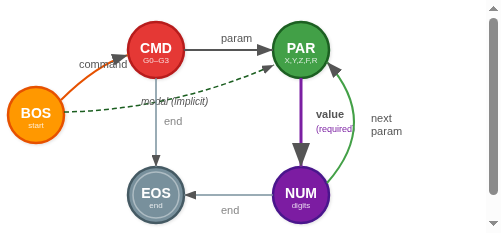
\includegraphics[width=0.75\columnwidth]{figures/type_fsm.png}
\caption{Type-transition FSM. After \textsc{Parameter}, only \textsc{Numeric} is valid (mandatory, bold edge); after \textsc{Numeric}, only \textsc{Parameter} or \texttt{EOS}. Modal persistence allows \texttt{BOS}~$\to$~\textsc{Parameter} directly (dashed). Each transition evaluates in $O(1)$. Command-specific constraints (Table~\ref{tab:core_commands}) further restrict valid parameters.}
\label{fig:grammar_constraints}
\end{figure}

\subsubsection{Soft Constraints as Training Penalties}

During training, soft penalty terms encourage compliance with domain-specific rules beyond hard syntactic constraints. These define a weighted regular language in which each rule $k$ penalizes violating sequences proportionally:
\begin{equation}
    \mathcal{L}_{\text{grammar}} = \sum_{k} \lambda_k \cdot \mathcal{L}_k
\end{equation}

\begin{table}[htbp]
\centering
\caption{Soft Grammar Constraint Penalties}
\label{tab:soft_constraints}
\small
\begin{tabular}{@{}lcp{3.8cm}@{}}
\toprule
\textbf{Constraint} & $\lambda$ & \textbf{Rule} \\
\midrule
Arc radius         & 1.0 & G2/G3 $\to$ predict R or I/J/K \\
Modal group        & 0.6 & One motion cmd per block \\
Rapid feed         & 0.5 & G0 $\to$ no F parameter \\
Arc alternation    & 0.4 & G2 $\leftrightarrow$ G3 in spirals \\
Cmd-param assoc.   & 0.4 & Valid params per command \\
Single letter      & 0.3 & No repeated addresses \\
Linear feed        & 0.3 & G1 $\to$ expect F \\
Z-retract pattern  & 0.2 & G0\,Z $\to$ XY reposition \\
\bottomrule
\end{tabular}
\normalsize
\end{table}

Weights reflect physical severity. An arc without radius ($\lambda=1.0$) produces an unexecutable instruction; the controller will fault. A rapid with feed rate ($\lambda=0.5$) is accepted by some controllers but semantically meaningless. Z-retract ordering ($\lambda=0.2$) is a stylistic convention, not a hard rule. These values derive from machining domain knowledge and have not been tuned by grid search. Two observations make the untuned weights acceptable in practice. First, hard masks enforce correctness at inference regardless, so the soft weights shape only the training-time gradient and cannot introduce grammar violations at generation. Second, the on/off ablation ($\mathcal{L}_{\text{grammar}} = 0$ vs.\ the full weighted sum, Section~\ref{sec:baseline_performance}) yields a $+1.0$-pp mean sequence-accuracy gain that is not statistically significant (paired post-hoc comparison vs.\ the full model, $p = 1.0$ after correction), suggesting that the published model's accuracy is not sensitive to the specific weight values. We interpret this as the soft constraints pulling the model toward domain-consistent parameter patterns during training but providing most of their operational value through the hard mask at inference time. A sensitivity sweep (e.g., randomized weight perturbations with paired-fold evaluation) is future work.

\subsubsection{When Constraints Can Hurt}

Hard constraints guarantee syntax but can propagate commitment errors. If the model is uncertain between \texttt{G1} and \texttt{G2}, choosing \texttt{G2} triggers the arc-radius requirement and forces an \texttt{R} prediction the model may not be prepared to make. Beam search with deferred commitment could mitigate this. Additionally, our grammar covers only G0--G3; valid constructs outside this subset would be incorrectly masked.

% ============================================================================
\section{Empirical Validation}
\label{sec:empirical}

We validate the framework's claims on 120 G-code files (62{,}403 lines total, 2{,}248 unique) from Autodesk Fusion~360 CAM, covering face milling, pocket milling, and adaptive clearing on a Bantam Tools desktop CNC mill. The empirical work serves two purposes:
\begin{itemize}[leftmargin=*, nosep]
    \item Section~\ref{sec:baseline_performance} establishes how the published hierarchical model compares to standard baselines (tokenizer comparison, grammar coverage, vocabulary growth, and downstream decoder performance).
    \item Sections~\ref{sec:design_space_exp}--\ref{sec:kl_measurement} \emph{test the definitions and the trichotomy} of Section~\ref{sec:design_space}: Experiments~A--D probe the three properties of Definitions~\ref{def:bounded}--\ref{def:grammar_valid} across seven tokenizer families and confirm Proposition~\ref{prop:trichotomy} cell-by-cell; Experiments~C and~E test what a trained decoder emits when free-generating under each tokenizer; and the KL-divergence measurement (Section~\ref{sec:kl_measurement}) tests whether grammar-constrained decoding under our framework distorts the model distribution in the regime ASAp~\cite{grammar_aligned} was designed for.
\end{itemize}

\paragraph{Canonical-line overlap between train and test splits.}
Because CAM-generated G-code is highly repetitive (62{,}403 raw lines collapse to 2{,}248 unique canonical forms, a 28:1 ratio; Section~\ref{sec:program_structure}), a large share of canonical lines that appear in a held-out test split also appear in the corresponding training split, even though the splits respect \emph{program} boundaries (no run from a held-out program leaks into training; Appendix~\ref{sec:repro_data}). We measured this directly across the 5 folds of the sensor-aligned experiment: mean canonical-line overlap rate between test and train is $93.6\%$ (range $79$--$100\%$ across folds). Experiments~C and~E should therefore be read as ``given a sensor window, reconstruct a canonical line the model has likely seen during training'' rather than ``given a sensor window, produce a novel canonical line.'' This is a realistic scenario for line-level process verification, where the task is to distinguish which of a small set of known canonical primitives is currently executing. It is, however, a weaker generalization test than the cross-operation OOV evaluation in Experiment~D (Section~\ref{sec:design_space_exp}), on which we rely for claims about novel geometry. Experiment~D uses disjoint \emph{operation types} for train and test and therefore measures how each tokenizer handles unseen coordinate values.

\subsection{Baseline performance}
\label{sec:baseline_performance}

We first establish how the published hierarchical model compares to standard baselines. On all 2{,}248 unique canonicalized lines, the hybrid tokenizer produces 2.5$\times$ fewer tokens than GPT-4's cl100k\_base BPE and 2.1$\times$ fewer than a BPE trained on our own corpus (Table~\ref{tab:tokenizer_comparison}); the domain-trained BPE learns useful merges such as keeping \texttt{G2} intact, but still fragments numeric coordinates and uses 903 vocabulary entries that scale with geometry. The hybrid tokenizer uses 19 fixed structural entries.

\begin{table}[htbp]
\centering
\caption{Tokenizer Comparison on 2{,}248 Unique G-Code Lines}
\label{tab:tokenizer_comparison}
\small
\begin{tabular}{@{}lrrr@{}}
\toprule
\textbf{Tokenizer} & \textbf{Total} & \textbf{Avg/line} & \textbf{Vocab used} \\
\midrule
GPT-4 (cl100k)            & 27{,}068 & 12.0 & 993 \\
GPT-2 (r50k)              & 27{,}153 & 12.1 & 715 \\
BPE-on-G-code$^{\ddagger}$ & 23{,}348 & 10.4 & 903 \\
Hybrid (ours)             & 10{,}922 & 4.9  & 19$^{\dagger}$ \\
\bottomrule
\multicolumn{4}{@{}l}{\scriptsize $^{\dagger}$Structural vocabulary; numeric values predicted by digit heads.}\\
\multicolumn{4}{@{}l}{\scriptsize $^{\ddagger}$BPE trained on our G-code corpus (vocab\,=\,975, min\,freq\,=\,2).}
\end{tabular}
\normalsize
\end{table}

The finite-state grammar of Section~\ref{sec:grammar} parses 99.9\% of the 2{,}248 unique toolpath lines (2{,}246/2{,}248; the two failures are preprocessing artifacts). The command distribution confirms that the four core motion commands dominate the corpus: G1 contributes 52.9\% of lines, implicit modal continuations 38.5\%, and G0/G2/G3 together 4.7\%, for a combined 96.1\% of all 62{,}403 lines.

Vocabulary growth approximately follows Heaps' law~\cite{heaps1978} with $V = kN^{\beta}$, $k \approx 620$, $\beta \approx 0.42$, $R^{2} = 0.95$ across 16 sampled file-count checkpoints (Table~\ref{tab:vocab_growth}). The flat vocabulary reaches 4{,}435 tokens after 120 files while the structural vocabulary remains fixed at 9, and the fit extrapolates to approximately 13{,}000 flat tokens at 1{,}000 files versus a constant 19 structural tokens. The fit is an approximation rather than a precise power law: the measured curve exhibits step changes at $N \approx 20$, $40$, and $110$ corresponding to new operation types and operating conditions entering the corpus, so we treat the Heaps' form as descriptive of the overall scaling trend rather than a precise model.

\begin{table}[htbp]
\centering
\caption{Cumulative Vocabulary Growth Across 120 Files (16 sampled checkpoints)}
\label{tab:vocab_growth}
\small
\begin{tabular}{@{}rrr@{}}
\toprule
\textbf{Files} & \textbf{Flat vocab.} & \textbf{Struct.}$^{\dagger}$ \\
\midrule
1   & 520   & 7 \\
5   & 1{,}326 & 7 \\
10  & 1{,}642 & 7 \\
15  & 1{,}669 & 7 \\
20  & 2{,}705 & 7 \\
25  & 2{,}836 & 7 \\
30  & 2{,}856 & 7 \\
40  & 3{,}371 & 8 \\
50  & 3{,}555 & 8 \\
60  & 3{,}579 & 8 \\
70  & 3{,}628 & 8 \\
80  & 3{,}630 & 8 \\
90  & 3{,}651 & 8 \\
100 & 3{,}683 & 8 \\
110 & 4{,}362 & 9 \\
120 & 4{,}435 & 9 \\
\bottomrule
\multicolumn{3}{@{}p{5.5cm}}{\scriptsize $^{\dagger}$Tokens observed in data; full structural vocabulary has 19 slots. Flat-vocabulary count includes both numeric and structural tokens (97--99\% numeric). Heaps' law fit across all 16 checkpoints: $V = 620 \cdot N^{0.42}$, $R^2 = 0.95$ (log--log). The curve shows step changes at $N \approx 20$, $40$, and $110$ corresponding to new operation types and operating conditions entering the corpus, so the smooth Heaps' form is an approximation rather than a precise fit.}
\end{tabular}
\normalsize
\end{table}

To evaluate whether the hierarchical tokenization yields usable predictions in practice, we trained a transformer decoder on a G-code reconstruction task in which the model reconstructs the G-code line that produced a given window of CNC sensor observations. The decoder uses 8 transformer layers, 12 attention heads, $d_{\text{model}} = 384$, dropout 0.1, and the multi-head loss of Eq.~\ref{eq:loss} with digit weight $\lambda_{d} = 15.0$, evaluated under 5-fold cross-validation on the same 120-file corpus. Table~\ref{tab:downstream} reports per-level accuracy. The hierarchical decomposition produces an accuracy gradient: structural levels (type, command, parameter) exceed 96\%, while numeric digit prediction at 91.1\% confirms that value prediction is the bottleneck.

\begin{table}[htbp]
\centering
\caption{Downstream Decoder Performance (5-Fold CV, teacher-forced: each prediction is conditioned on the ground-truth prefix). \emph{Mean} is the 5-fold test-set mean; \emph{Best Fold} is the per-head maximum across the five test folds. Values are the released \texttt{v7\_best\_5fold} multi-head decoder checkpoints (Appendix~\ref{sec:reproducibility}).}
\label{tab:downstream}
\small
\begin{tabular}{@{}lcc@{}}
\toprule
\textbf{Prediction Level} & \textbf{Mean} & \textbf{Best Fold} \\
\midrule
Token (overall)              & 94.7\% & 97.4\% \\
Sequence (exact match)       & 84.4\% & 89.2\% \\
Type ($\tau$)                & 98.8\% & 99.7\% \\
Command ($\iota_{\text{cmd}}$) & 98.3\% & 100\% \\
Parameter ($\iota_{\text{par}}$) & 97.2\% & 98.7\% \\
Numeric (digits)             & 91.1\% & 94.4\% \\
\bottomrule
\end{tabular}
\normalsize
\end{table}

An ablation on the soft grammar-constraint penalties ($\mathcal{L}_{\text{grammar}} = 0$) yields mean sequence accuracy of 85.1\% versus 86.1\% for the full model in the same ablation suite, a modest 1.0-point gain that is not statistically significant across folds (paired post-hoc comparison vs.\ the full model, $p = 1.0$ after correction; uncorrected $p = 0.094$, Cohen's $d \approx -1.0$). This is consistent with our observation in Section~\ref{sec:constrained_decoding} that hard constraints can propagate commitment errors: the soft penalties help slightly but are not the dominant factor in sequence-level accuracy.

A second ablation isolates the contribution of the structured decomposition itself. We retrain the flat 712-class token head \emph{alone}, with the auxiliary type, command, parameter, and digit losses removed (their weights set to zero) and the same recipe, frozen encoder, and five folds, and compare it to the full multi-head model under identical settings. The flat-only decoder reaches a mean token accuracy of only $75.0\%$ versus $94.9\%$ for the full model, a $+19.9$-pp gap (the full-model figure reproduces the released model's $94.7\%$ in Table~\ref{tab:downstream}). The effect is primarily one of \emph{training stability}. Without the auxiliary decomposition the flat decoder trains successfully on three folds ($94.5$--$97.2\%$ token) but collapses to a degenerate, near-constant output on the other two ($\approx\!44\%$ token, $0\%$ sequence exact-match), inflating the cross-fold standard deviation to $25$~pp. The auxiliary structural heads therefore act as a multi-task regularizer that keeps the flat 712-way prediction problem learnable on this small ($\sim\!300$-sample-per-fold) dataset, rather than as a uniform accuracy increment. Per-fold values and the run configuration are released in \texttt{flat\_vs\_structured\_results.json}.

\subsection{Testing the three properties (Experiments A, B, D)}
\label{sec:design_space_exp}

This subsection tests Definitions~\ref{def:bounded}--\ref{def:grammar_valid} and Proposition~\ref{prop:trichotomy} directly by populating every cell of Table~\ref{tab:design_space} with a real measurement on the 120-file corpus. Each experiment maps one-to-one onto a definition:
\begin{itemize}[leftmargin=*, nosep]
    \item Experiment~A tests Definition~\ref{def:bounded} (\textsc{Bounded}) by measuring active vocabulary growth on every tokenizer family.
    \item Experiment~B tests Definition~\ref{def:lossless} (\textsc{Lossless}) by measuring coordinate roundtrip error.
    \item Experiment~D tests the operational consequence of failing \textsc{Bounded} on novel geometries by measuring held-out OOV across cross-geometry splits.
\end{itemize}
The test of property~(i) of Definition~\ref{def:grammar_valid} (\textsc{Grammar}) requires a trained model and is deferred to Section~\ref{sec:exp_c}.

\paragraph{Experiment A: Vocabulary growth.}
For each tokenizer we walk the 120 \texttt{*\_aligned.csv} files in lexical order and record the cumulative number of distinct token ids actually emitted on encode (active vocabulary). Pretrained tokenizers (GPT-4, GPT-2) have fixed capacity but their active vocabulary grows as new substrings are observed; data-trained tokenizers (Domain BPE, WordPiece, Flat per-value) build vocabulary as they encounter the corpus. Table~\ref{tab:exp_a_growth} reports the active vocabulary at four file counts.

\begin{table}[htbp]
\centering
\caption{Experiment~A: Cumulative Distinct Token Types Observed (Vocabulary Growth)}
\label{tab:exp_a_growth}
\scriptsize
\begin{tabular}{@{}lrrrr@{}}
\toprule
\textbf{Tokenizer} & \textbf{1} & \textbf{20} & \textbf{60} & \textbf{120} \\
\midrule
Hierarchical (ours) & 22 & 22 & 25 & 25 \\
GPT-4 BPE (cl100k) & 377 & 908 & 964 & 993 \\
GPT-2 BPE (r50k) & 293 & 619 & 671 & 715 \\
Character-level & 20 & 25 & 26 & 26 \\
Flat per-value & 520 & 2,705 & 3,579 & 4,435 \\
Domain BPE & 325 & 798 & 923 & 993 \\
WordPiece & 389 & 774 & 865 & 929 \\
\bottomrule
\multicolumn{5}{@{}l}{\scriptsize Columns are file count; cells are cumulative distinct token ids emitted.}
\end{tabular}
\normalsize
\end{table}


The hierarchical tokenizer and character-level tokenizer plateau immediately at 25 and 26 active tokens respectively. The 25 for hierarchical reflects the small structural alphabet (Table~\ref{tab:vocab_complete}: 7--9 tokens active in this dataset) plus the 11-element digit/sign sub-vocabulary that the model emits. Table~\ref{tab:tokenizer_comparison} reports only the 19 structural slots: numeric values are predicted by the digit heads rather than vocabulary entries (Section~\ref{sec:decomposition}). The two counts are consistent under different definitions of ``vocabulary.'' The BPE and WordPiece variants are nominally bounded but use 700--993 active tokens, roughly $40\times$ the structural vocabulary needed by Definition~\ref{def:bounded}. The flat per-value tokenizer grows monotonically from 520 to 4{,}435 tokens across 120 files with no sign of saturation; the curve approximately follows Heaps' law~\cite{heaps1978} with $\beta \approx 0.42$ across 16 sampled checkpoints (Table~\ref{tab:vocab_growth}). \textsc{Bounded} therefore holds for every row except flat per-value, as Proposition~\ref{prop:trichotomy} predicts.

\paragraph{Experiment B: Coordinate reconstruction (in-distribution sanity).}
We extract every unique \emph{(address, value)} pair from the canonicalized corpus (4{,}418 pairs across X/Y/Z/R/F) and round-trip each value through every tokenizer's encode--decode. Table~\ref{tab:exp_b_recon} reports the mean absolute reconstruction error in the address's native unit.

\begin{table}[htbp]
\centering
\caption{Experiment~B: Mean Coordinate Reconstruction Error (in; in/min for F)}
\label{tab:exp_b_recon}
\scriptsize
\begin{tabular}{@{}lrrrrr@{}}
\toprule
\textbf{Tokenizer} & \textbf{X} & \textbf{Y} & \textbf{Z} & \textbf{R} & \textbf{F} \\
\midrule
Hierarchical (ours) & 0.0002 & 0.0002 & 0.0003 & 4.4e-17 & 0.3000 \\
GPT-4 BPE (cl100k) & 0 & 0 & 0 & 0 & 0 \\
GPT-2 BPE (r50k) & 0 & 0 & 0 & 0 & 0 \\
Character-level & 0 & 0 & 0 & 0 & 0 \\
Flat per-value & 0 & 0 & 0 & 0 & 0 \\
Domain BPE & 0 & 0 & 0 & 0 & 0 \\
WordPiece & 0.0026 & 0.0027 & 0.0023 & 0.0003 & 0 \\
\bottomrule
\end{tabular}
\normalsize
\end{table}


This experiment serves as a sanity check rather than a differentiator: encode--decode is symbolically lossless for every tokenizer that retains the input string verbatim, so BPE variants, character-level, and flat per-value all achieve zero error on values that already appear in the training corpus. Our hierarchical tokenizer attains a mean error of $\approx\!0.00025\,$in ($6.4\,\mu$m) on X/Y/Z, close to the $p/4$ mean expected for uniformly distributed quantization error at $p = 0.001\,$in and within the $p/2$ worst-case bound; the residual is quantization-induced rather than a tokenization failure, and remains below the mill's positional accuracy ($\approx\!10\,\mu$m). WordPiece exhibits a small but non-zero reconstruction error ($\approx\!0.0025\,$in, $\approx\!64\,\mu$m mean) attributable to whitespace normalization in the HuggingFace decoder. The differentiator between tokenizers is not in-distribution roundtrip but cross-distribution generalization, which Experiment~D addresses directly.

\paragraph{Experiment D: Cross-geometry OOV (the principal experiment).}
We split the corpus by operation type---face milling, pocket milling, and adaptive clearing---and for each fold ``train'' the tokenizer on two operations and evaluate on the third. For tokenizers without an explicit training step, we instead populate the active vocabulary by encoding the training fold and then count, on the held-out fold, how many emitted token ids fall outside the seen vocabulary. Table~\ref{tab:exp_d_oov} reports the held-out OOV rate.

\begin{table}[htbp]
\centering
\caption{Experiment~D: Held-Out Operation OOV Rate (\%)}
\label{tab:exp_d_oov}
\scriptsize
\begin{tabular}{@{}lrrr@{}}
\toprule
\textbf{Tokenizer} & \textbf{adaptive} & \textbf{face} & \textbf{pocket} \\
\midrule
Hierarchical (ours) & 0.000 & 0.001 & 0.000 \\
GPT-4 BPE (cl100k) & 4.810 & 0.250 & 0.384 \\
GPT-2 BPE (r50k) & 2.536 & 0.048 & 0.399 \\
Character-level & 0.002 & 0.000 & 0.000 \\
Flat per-value & 65.421 & 18.090 & 29.852 \\
Domain BPE & 0.949 & 0.025 & 0.061 \\
WordPiece & 2.142 & 0.047 & 0.065 \\
\bottomrule
\end{tabular}
\normalsize
\end{table}


The ranking is unambiguous. The hierarchical and character-level tokenizers achieve essentially zero OOV across all folds; both decompose unseen values into a finite alphabet that is closed under composition. Domain-trained BPE and WordPiece remain in single-digit-percent territory but are not OOV-free; GPT-4's BPE reaches 4.81\% on held-out adaptive operations (which contain the most geometrically diverse coordinates), and the flat per-value tokenizer collapses entirely (18--65\% OOV across folds). This is the empirical signature of Proposition~\ref{prop:trichotomy}: any tokenizer that satisfies bounded vocabulary by enumerating values (flat) or by data-driven subword merges (BPE/WordPiece) loses lossless representation on novel geometries, while only digit-decomposed and character-level tokenizers preserve it. Of those two, only the hierarchical decomposition also satisfies grammar validity at the value level (Definition~\ref{def:grammar_valid}, property~(ii)), since character-level FSAs over digit strings explode combinatorially before grammar productions can attach.

Together, Experiments~A, B, and~D populate every cell of the design-space table and confirm that the (\textsc{Bounded}, \textsc{Lossless}, \textsc{Grammar}) corner is occupied by exactly one row.

\subsection{Free-generation grammar validity (Experiment C)}
\label{sec:exp_c}

This subsection tests property~(i) of Definition~\ref{def:grammar_valid}: whether a trained decoder under each tokenizer family can produce encodings that decode back to grammatical lines. Experiments~A and~D establish what each tokenizer \emph{can} represent in principle; Experiment~C measures what a trained model actually emits when freely generating new lines.

We train one decoder per tokenizer family on each of the five v7 cross-validation folds (per-fold test counts 132/113/106/108/93, 552 evaluated samples in total; the corresponding train and validation splits also vary by fold). Every arm uses an identical \texttt{FlatVocabDecoder} architecture (192-dim, 4 layers, 8 heads), the same pre-cached encoder memory (sensor\_dim $= 256$), and the same vanilla cross-entropy training schedule (Adam, 80 epochs, lr $3{\times}10^{-4}$, dropout 0.3, batch size 32).

\textbf{The hierarchical row uses the same 712-token vocabulary as the published baseline but is retrained with this slim trainer.} This is intentional. A cross-tokenizer comparison is only meaningful if every row is trained identically, so we strip out the focal loss, scheduled sampling, label smoothing, and heavy ($15\times$) digit weighting that the published model relies on, \emph{and} we replace the published model's hierarchical three-head cascade with a single flat softmax over the 712-token vocabulary (the same \texttt{FlatVocabDecoder} architecture used by every other row). The slim ``hierarchical'' row is therefore a flat decoder over the hybrid 712-token vocabulary. Its gap to the published $94.7\%$ has two sources: (a) the training recipe (scheduled sampling, focal loss, label smoothing, and $15\times$ digit weighting vs.\ vanilla cross-entropy) and (b) the architecture (multi-head cascade vs.\ flat softmax). We do not decompose the gap because it would require retraining the published model's architecture under the slim schedule, which is the opposite of what this comparison is designed to do.

For reference, the mean slim-trainer test token accuracy across folds is (as percentages, mean $\pm$ std): Domain BPE (whitespace) $89.07 \pm 1.74$, Domain BPE (byte-level) $90.59 \pm 2.72$, WordPiece $89.38 \pm 2.43$, character-level $93.79 \pm 1.26$, flat per-value $82.11 \pm 3.01$, GPT-4 compact $91.58 \pm 1.92$, and hierarchical (slim flat) $85.03 \pm 3.57$. Sequence-level exact-match accuracy is tightly clustered at $48$--$53\%$ across all rows and is not discriminative. Within the slim regime, token-accuracy differences between tokenizers are modest and do not predict the grammar-validity ranking: character-level has the highest slim token accuracy, while whitespace-pre-tokenized BPE remains $89\%$ accurate at the token level yet produces $0\%$ grammatically valid output, so the sub-case~2a failure is invisible at the token-accuracy level. The grammar-validity behavior reported in Table~\ref{tab:exp_c} is therefore a structural property of the tokenizer and decoder pair, not a proxy for model accuracy.

For each test sample we free-generate one G-code line conditioned on its sensor memory (no teacher forcing, temperature~$=1.0$, no top-$k$), decode the generated id sequence back to text via the tokenizer's native \texttt{decode}, and check whether the decoded line is syntactically valid against the regular grammar of Section~\ref{sec:formal_grammar}. Table~\ref{tab:exp_c} reports the grammar-validity rate aggregated across all five folds.

\begin{table}[htbp]
\centering
\caption{Experiment~C: Free-Generation Grammar Validity (5-fold mean $\pm$ std)}
\label{tab:exp_c}
\scriptsize
\begin{tabular}{@{}lr@{}}
\toprule
\textbf{Tokenizer} & \textbf{Grammar valid (\%)} \\
\midrule
Domain BPE (whitespace pre-tokenizer) & $0.00 \pm 0.00$ \\
Domain BPE (byte-level pre-tokenizer) & $97.14 \pm 1.55$ \\
WordPiece                             & $0.00 \pm 0.00$ \\
Character-level                       & $97.64 \pm 3.47$ \\
Flat per-value                        & $96.98 \pm 1.72$ \\
GPT-4 BPE (compact)                   & $97.09 \pm 2.39$ \\
\midrule
\textbf{Hierarchical (ours)}          & $\boldsymbol{98.31 \pm 1.38}$ \\
\bottomrule
\multicolumn{2}{@{}p{0.9\columnwidth}}{\scriptsize 5-fold cross-validation, per-fold test counts 132/113/106/108/93 (552 samples total per row). Ground-truth lines pass our grammar check at 95.8\% on average; the gap reflects rare auxiliary lines outside our regular grammar fragment. The hierarchical row is the slim-trainer reproduction described above; the published model achieves 99.9\% grammar coverage on the full corpus (Section~\ref{sec:empirical}). The byte-level BPE row is the reviewer-requested control that replaces the HuggingFace \texttt{Whitespace} pre-tokenizer and decoder with \texttt{ByteLevel}; canonical-input roundtrip is bit-exact on this variant.}
\end{tabular}
\normalsize
\end{table}

The result separates into two groups. Domain BPE with the standard \texttt{Whitespace} pre-tokenizer and WordPiece collapse to $0.00 \pm 0.00\%$ grammar validity across 552 test samples and 5 independent folds, never producing a single grammatically valid line. Every other tokenizer, including a byte-level BPE control trained on the same corpus, reaches 96--98\%.

\paragraph{Statistical significance.} Within the non-failing group the differences are small. A paired bootstrap over the 5 folds (10{,}000 resamples, seed 42) finds that the hierarchical row is not significantly better than byte-level BPE, character-level, or GPT-4 compact (one-sided $p = 0.153$, $0.235$, $0.118$ respectively); the $+1.33$-pp gap over flat per-value is marginally significant ($p = 0.016$, $95\%$ CI $[+0.08, +2.43]$ pp). The gap over the two failing tokenizers is significant at $p < 10^{-4}$. Among the tokenizers whose decoders preserve numeric contiguity, grammar validity saturates near the $95.8\%$ ground-truth ceiling, and the differences between rows are within fold-level noise.

The failure mode for the standard BPE row is sub-case~2a of the case analysis in Section~\ref{sec:impossibility}, a deterministic decode-side failure rather than an intrinsic limitation of BPE merges. Inspection of generated samples shows that the model correctly predicts the subwords for values such as $1.4919$; the HuggingFace BPE decoder, inverting the \texttt{Whitespace} pre-tokenizer, then reassembles those subwords with whitespace at every BPE boundary, producing \texttt{"G0 X1 . 4919 Y1 . 4848"} instead of \texttt{"G0 X1.4919 Y1.4848"}. A regex-based G-code parser rejects the spaced version even though every subword is correct.

The byte-level BPE control isolates sub-case~2a from sub-case~2b (merge-table ambiguity). Replacing the \texttt{Whitespace} pre-tokenizer and decoder with \texttt{ByteLevel} makes the encode--decode roundtrip bit-exact on the canonicalized input: a freshly trained byte-level BPE round-trips \texttt{R0.1755} to \texttt{R0.1755} with no whitespace artifact. Under that configuration, grammar validity rises to $97.14 \pm 1.55\%$, statistically indistinguishable from the other non-fragmenting tokenizers. This is a negative result for sub-case~2b: the merge table's context-dependent fragmentation does not cause grammar failure in practice on our corpus. We therefore read Table~\ref{tab:exp_c} as evidence that the BPE failure in standard deployments is a decoder-configuration issue with a known fix, not a property of subword tokenization as a class. Case~2 of Proposition~\ref{prop:trichotomy} reduces accordingly: the out-of-the-box BPE pipelines used in practice (with a \texttt{Whitespace} pre-tokenizer) deterministically fail Definition~\ref{def:grammar_valid} property~(i), while a non-standard byte-level configuration passes on this corpus. Byte-level BPE still fails Definition~\ref{def:bounded} in practice (100--1000 learned merges that grow with geometry) and the value-level form of Definition~\ref{def:grammar_valid} property~(ii), for the structural reason established in Section~\ref{sec:impossibility}, so the all-checkmarks corner of Table~\ref{tab:design_space} remains occupied only by digit decomposition; byte-level BPE improves on the whitespace variant but does not satisfy all three properties simultaneously.

Table~\ref{tab:c_samples} makes the failure mode visible with free-generated outputs from all six tokenizer families on three ground-truth test lines. The four non-fragmenting tokenizers (char-level, flat per-value, GPT-4 compact, hierarchical) reproduce parseable G-code, while Domain BPE and WordPiece consistently insert whitespace between the address letter, the integer part, the decimal point, and the fractional part, even when the underlying value is correct.

\begin{table}[htbp]
\centering
\caption{Free-Generated Samples by Tokenizer Family (test fold~1)}
\label{tab:c_samples}
\small
\begin{tabular}{@{}lp{4.7cm}c@{}}
\toprule
\textbf{Tokenizer} & \textbf{Predicted line} & \textbf{Parses?} \\
\midrule
\multicolumn{3}{@{}l}{\emph{GT: \texttt{Y0.1755}}} \\
Domain BPE          & \texttt{Y0 . 1755}  & $\times$ \\
WordPiece           & \texttt{Y2 . 9132}  & $\times$ \\
Character-level     & \texttt{Y0.1755}    & $\checkmark$ \\
Flat per-value      & \texttt{Y0.1755}    & $\checkmark$ \\
GPT-4 BPE (compact) & \texttt{Y0.1755}    & $\checkmark$ \\
Hierarchical (ours) & \texttt{X0.596}     & $\checkmark$ \\
\midrule
\multicolumn{3}{@{}l}{\emph{GT: \texttt{G0 X1.4919 Y1.4848}}} \\
Domain BPE          & \texttt{X1 . 4561 Y1 . 5749 R0 . 1188} & $\times$ \\
WordPiece           & \texttt{G1 X1 . 4919 Y1 . 4848}        & $\times$ \\
Character-level     & \texttt{G0 X1.4919 Y1.4848}            & $\checkmark$ \\
Flat per-value      & \texttt{X1.4561 Y1.5749 R0.1188}       & $\checkmark$ \\
GPT-4 BPE (compact) & \texttt{G0 X1.4919 Y1.4848}            & $\checkmark$ \\
Hierarchical (ours) & \texttt{G0 X1.492 Y1.485}              & $\checkmark$ \\
\midrule
\multicolumn{3}{@{}l}{\emph{GT: \texttt{X1.4561 Y1.5749 R0.1188}}} \\
Domain BPE          & \texttt{X1 . 4561 Y1 . 5749 R0 . 1188} & $\times$ \\
WordPiece           & \texttt{X1 . 4561 Y1 . 5749 R0 . 1188} & $\times$ \\
Character-level     & \texttt{G0 X1.4919 Y1.4848}            & $\checkmark$ \\
Flat per-value      & \texttt{G1 X3.275}                     & $\checkmark$ \\
GPT-4 BPE (compact) & \texttt{X1.4561 Y1.5749 R0.1188}       & $\checkmark$ \\
Hierarchical (ours) & \texttt{G0 X1.492 Y1.485}              & $\checkmark$ \\
\bottomrule
\end{tabular}

\smallskip
{\small ``Parses?'' indicates whether the predicted line passes the regular grammar of Section~\ref{sec:formal_grammar}. The third row of the first GT block is the decisive evidence: Domain BPE has predicted \emph{exactly} the right value (\texttt{0.1755}), but the decoder's whitespace insertion makes the result unrecognizable to a G-code parser. The same model under any tokenizer that does not split numeric strings into BPE subwords successfully emits the same value as a parseable line.}
\end{table}

This is the failure of Definition~\ref{def:grammar_valid} property~(i) under a standard BPE pipeline: whitespace reinserted between subword pieces makes value-level reconstruction ambiguous. Character-level, flat per-value, GPT-4 compact, and the byte-level BPE control survive because their decode operations preserve the contiguous numeric string. The hierarchical tokenizer survives by construction, since digit predictions compose deterministically into a valid \texttt{X<value>} word regardless of which digit head is fired. The distinction Table~\ref{tab:exp_c} supports is between tokenizers whose decoder preserves numeric contiguity and tokenizers whose decoder inserts whitespace between learned subwords, not between BPE and non-BPE per se.

\subsection{Toolpath reconstruction error (Experiment E)}
\label{sec:exp_e}

Experiment~C tests property~(i) of Definition~\ref{def:grammar_valid} at the symbolic level, asking whether decoded outputs parse. Experiment~E measures the downstream consequence of grammar failure in physical units: how far the toolpath implied by a free-generated line deviates from the ground-truth toolpath. For each test sample, we parse both the ground-truth and free-generated lines through the same \texttt{GCodeToCoordinateParser}~(Section~\ref{sec:related}), reconstruct the implied 3D toolpath, and compute the bidirectional Hausdorff distance between the two point sets:
\[
H(A, B) = \max\!\Big(\sup_{a \in A}\inf_{b \in B}\|a-b\|,\;\sup_{b \in B}\inf_{a \in A}\|a-b\|\Big).
\]
The parser treats both \texttt{G0} and \texttt{G1} as linear interpolation between the prior and next endpoints.\footnote{Real CNC controllers typically execute \texttt{G0} rapid traversals with independent-axis motion rather than coordinated linear interpolation, which produces a ``dog-leg'' path that deviates from a straight line by up to $\sqrt{2}\cdot d/2$ at the midpoint of a diagonal move of length $d$. Our linear-interpolation approximation is consistent with how most simulators and CAM previews render \texttt{G0} and does not affect the grammar-validity metric (Experiment~C), which is evaluated at the symbolic level before any geometric reconstruction. It may introduce a small systematic bias in the Experiment~E Hausdorff distances, but the bias is common across all tokenizer rows and therefore does not affect the cross-tokenizer ranking.}
Table~\ref{tab:exp_e} reports the per-tokenizer mean, median, and 95th-percentile Hausdorff distance in inches, aggregated across all five cross-validation folds.

\begin{table}[htbp]
\centering
\caption{Experiment~E: Toolpath Hausdorff Distance from Free-Generated Output (inches, 5-fold mean $\pm$ std)}
\label{tab:exp_e}
\scriptsize
\begin{tabular}{@{}lrrr@{}}
\toprule
\textbf{Tokenizer} & \textbf{Mean} & \textbf{Median} & \textbf{p95} \\
\midrule
Domain BPE (whitespace) & $1.322 \pm 0.152$ & $0.637 \pm 0.095$ & $3.331 \pm 0.063$ \\
Domain BPE (byte-level) & $1.432 \pm 0.122$ & $0.317 \pm 0.155$ & $3.535 \pm 0.000$ \\
WordPiece               & $1.311 \pm 0.180$ & $0.620 \pm 0.122$ & $3.258 \pm 0.166$ \\
Character-level         & $1.277 \pm 0.136$ & $\boldsymbol{0.163 \pm 0.068}$ & $3.535 \pm 0.000$ \\
Flat per-value          & $1.319 \pm 0.223$ & $0.211 \pm 0.262$ & $3.493 \pm 0.095$ \\
GPT-4 BPE (compact)     & $1.342 \pm 0.158$ & $0.264 \pm 0.200$ & $3.493 \pm 0.095$ \\
\midrule
\textbf{Hierarchical (ours)} & $1.529 \pm 0.042$ & $0.473 \pm 0.169$ & $3.535 \pm 0.000$ \\
\bottomrule
\multicolumn{4}{@{}p{0.95\columnwidth}}{\scriptsize p95 saturates near 3.5\,in---the bidirectional Hausdorff between the two extreme positions in the test set's coordinate range---because samples whose generation collapses default to that bound. Median is the more discriminative statistic. As in Experiment~C, the hierarchical row is the slim-trainer reproduction; the published multi-head model is expected to dominate, but is omitted here to keep the cross-tokenizer comparison clean.}
\end{tabular}
\normalsize
\end{table}

The mean and p95 cluster across all tokenizers because the test set contains a small number of geometrically diverse samples on which every slim-trainer model produces poor reconstructions; these dominate the upper percentiles. The discriminative statistic is the \emph{median}, where two groups emerge:
\begin{itemize}[leftmargin=*, nosep]
    \item Tokenizers that pass Experiment~C (byte-level BPE, character-level, flat per-value, GPT-4 compact, hierarchical) achieve median Hausdorff between $0.16$ and $0.47$\,in. The tightest median is char-level at $0.163$\,in; the hierarchical slim-trainer row sits at $0.473$\,in, reflecting its lower absolute token accuracy in the slim regime rather than a tokenizer-side disadvantage.
    \item Tokenizers that fail Experiment~C (Domain BPE with whitespace pre-tokenizer, WordPiece) sit at median $0.62$--$0.64$\,in, roughly $2$--$4\times$ larger than the non-failing group, because their malformed outputs cannot be parsed into points at all and the parser falls back to the start position.
\end{itemize}
The grammar-failure penalty is therefore not confined to syntax: it propagates directly into centimetre-scale median toolpath error per line and compounds over a multi-thousand-line program. The byte-level BPE row joins the non-failing group (median $0.317$\,in), confirming that the toolpath-error gap is explained by decoder-side whitespace reinsertion rather than by BPE's merge table.

Experiments~C and~E isolate the tokenizer's contribution under fixed training conditions. Across all 5 folds, the tokenizers that fragment coordinate strings at decode time were unrecoverable at generation time regardless of how well the model itself learned, and the 5-fold standard deviations on the BPE/WordPiece grammar-validity rate ($0.00 \pm 0.00$) confirm a deterministic structural failure rather than a fold-dependent artifact. Because the failure lies in the decode rule rather than in the model or the data, we expect the same outcome for any tokenizer that fragments coordinate strings.

\subsection{Distribution distortion under grammar masking}
\label{sec:kl_measurement}

Park et al.~\cite{grammar_aligned} show that na\"ive grammar-constrained decoding can distort the underlying model distribution and propose ASAp as a corrective. To check whether this concern is operationally relevant for our system, we measure the per-step KL divergence between the model's grammar-masked and unmasked type-head distributions on the held-out test sets across all five cross-validation folds. At each non-pad position $t$, we compute
\[
\text{KL}_t = \mathrm{KL}\!\left(\mathrm{softmax}(\ell_t + M_t)\,\|\,\mathrm{softmax}(\ell_t)\right),
\]
where $\ell_t \in \mathbb{R}^4$ are the type-head logits and $M_t$ is the DFA-derived type-level mask from Section~\ref{sec:formal_grammar}. We also report the \emph{blocked probability mass}: the share of the unmasked distribution that lies on grammar-disallowed types.

\begin{table}[htbp]
\centering
\caption{KL Divergence between Grammar-Masked and Unmasked Type Distributions (5-Fold)}
\label{tab:kl_distortion}
\scriptsize
\begin{tabular}{@{}lccc@{}}
\toprule
\textbf{Fold} & \textbf{KL$(P_{\mathrm{m}}\!\|\!P_{\mathrm{u}})$} (nats) & \textbf{Blocked mass} & \textbf{Positions} \\
\midrule
1 & 0.0031 & 0.0016 & 1{,}509 \\
2 & 0.0004 & 0.0004 & 1{,}331 \\
3 & 0.0098 & 0.0020 & 1{,}302 \\
4 & 0.0067 & 0.0019 & 1{,}296 \\
5 & 0.0053 & 0.0012 & 1{,}130 \\
\midrule
\textbf{Mean $\pm$ std} & $\boldsymbol{0.0051 \pm 0.0032}$ & $\boldsymbol{0.0014}$ & 6{,}568 total \\
\bottomrule
\end{tabular}
\normalsize
\end{table}

The mean KL divergence of $0.005$ nats ($\approx 0.007$ bits) is negligible: it corresponds to a multiplicative shift factor of $\exp(0.005) \approx 1.005$ on the most-affected token's probability. The unmasked model already places $99.86\%$ of its type-prediction mass on grammar-valid types (a consequence of training under the type-head loss with implicit grammar exposure), so the mask removes only the residual $0.14\%$. ASAp-style corrective methods are designed for the regime in which a substantial share of the unmasked model's probability mass falls on grammar-disallowed tokens; our observed blocked-mass fraction is two orders of magnitude smaller than that. This empirically supports our $O(1)$ hard-mask design choice (Section~\ref{sec:constrained_decoding}) and confirms that, for grammars whose transitions are near-deterministic given a sufficiently trained model, the Park~et~al.\ critique is muted in practice. This measurement is on the four-way type head, where transitions are most deterministic and a low KL is therefore expected; we do not separately quantify distortion from the value-level masks (the \texttt{R}-required boost and the no-repeat-address and \texttt{G0}-no-F masks), which act on the identity and digit heads, so the claim is properly read as ``type-level transition distortion is negligible.'' The reported $\pm$ is the population standard deviation across the five folds.

% ============================================================================
\section{Discussion}
\label{sec:discussion}

G-code separates into a structural component (type, command, parameter identity) that is small and discrete, and a numeric component (coordinate values) that is continuous and unbounded. The two components demand different mechanisms. In the downstream results, structural predictions exceed 96\% accuracy while numeric digit prediction reaches 91.1\% (Table~\ref{tab:downstream}); we read this five-point gap as support for the decomposition. Existing systems conflate the two. GLLM~\cite{gllm} applies uniform BPE over both commands and coordinates, and Image2Gcode~\cite{image2gcode} treats everything as continuous. The same separation should apply to any numeric-heavy domain-specific language, including robot motion programs, 3D printer instructions, PLC ladder logic, and other CNC dialects.

The framework extends Technical Language Processing from human-written prose to formally specified machine languages. Prior TLP work~\cite{tlp_cleaning,tlp_keyword,tlp_semiautonomous,tlp_nuclear,tlp_fault,tlp_foundational,tlp_adapting} addresses lexical failure modes in maintenance logs, equipment reports, and fault summaries, where the challenge is jargon, abbreviation, and inconsistent terminology. G-code is formally specified, machine generated, and numerically dense, and its tokenization failure is structural rather than lexical (Table~\ref{tab:tlp_comparison}). Whether G-code is representative of a broader category that includes RAPID, KRL, PLC structured text, and STEP-NC, or an outlier among formally specified technical languages, requires investigation across multiple languages.

BPE behaves differently under its two pre-tokenizer configurations (Section~\ref{sec:exp_c}). Standard whitespace-pre-tokenized BPE and WordPiece collapse to $0.00 \pm 0.00\%$ free-generation grammar validity across 5 folds; byte-level BPE, trained on the same corpus with the same vocabulary budget, recovers to $97.14\%$, statistically indistinguishable from the non-fragmenting rows. The merge-table ambiguity that Proposition~\ref{prop:trichotomy}'s Case~2 argued would cause grammar failure (sub-case~2b) does not materialize on our corpus; the observed failure lies entirely in the decoder configuration (sub-case~2a). This narrows what the BPE critique supports. The all-checkmarks corner of Table~\ref{tab:design_space} is still occupied only by digit decomposition, but through a different discriminator. Byte-level BPE satisfies Definition~\ref{def:grammar_valid} property~(i) yet fails Definition~\ref{def:bounded} (its active vocabulary grows with geometry) and the value-level form of property~(ii) (no consistent token boundary at which to apply a per-value constraint mask).

\paragraph{Limitations.}
\textbf{Grammar scope.} The grammar covers only the four core motion commands (G0--G3) with five parameter addresses (\texttt{X}, \texttt{Y}, \texttt{Z}, \texttt{F}, \texttt{R}). A production system would need the \texttt{I}/\texttt{J}/\texttt{K} arc-center format (the default on many controllers, and required for arcs exceeding $180^\circ$), canned cycles (\texttt{G81}--\texttt{G89}), tool compensation (\texttt{G41}/\texttt{G42}), coordinate systems beyond \texttt{G54}, tool management, and controller-specific dialects (Fanuc, Siemens, Mazak, Haas).

\textbf{Machine envelope and precision.} The dataset comes from a desktop-class 3-axis mill with a $\sim$140$\times$102$\times$60\,mm work envelope, and the per-parameter precision in Table~\ref{tab:precision} is chosen accordingly ($0.001$\,in on \texttt{X}/\texttt{Y}/\texttt{Z}; $0.0001$\,in on \texttt{R}). Production CNC work routinely involves larger ranges ($\pm 2000$\,mm on gantry mills), finer nominal precisions ($0.1\,\mu$m in aerospace finishing), or coarser ones ($0.1$\,mm in woodworking). The digit-head configuration scales by adjusting the integer- and decimal-digit counts per address in Table~\ref{tab:precision} without structural changes to the framework, but we have not evaluated this empirically.

\textbf{Firmware scope.} The canonicalizer is firmware-agnostic; Section~\ref{sec:tokenization} shows that variable-precision strings like \texttt{X3.2} and \texttt{X3.2000} collapse to the same token bucket under both TinyG (the controller on our Bantam mill) and grbl. We have not tested against Fanuc, Siemens, Haas, or Mazak dialects, which use different comment syntaxes, subroutine conventions, and modal group definitions.

\textbf{Digit independence.} The independence assumption is justified for later decimal positions (mutual information $< 0.2$ bits) but breaks down at the integer-decimal boundary ($d_{1}$--$d_{2}$: 0.85 bits); a partial autoregressive chain could address this.

\textbf{Dataset scope.} The grammar coverage evaluation uses the same dataset from which the grammar was designed, so 99.9\% coverage is descriptive of this corpus, not predictive of unseen CAM output. Held-out evaluation across CAM systems (Mastercam, SolidCAM) and controllers is needed to assess generalization. Canonical-line overlap between train and test splits averages $93.6\%$ across folds (Section~\ref{sec:empirical}), so Experiments~C and~E should be read as verification rather than novel-line generation. The held-out OOV experiment (Experiment~D) uses disjoint operation types and provides the principal generalization test.

\textbf{Soft-constraint weights.} The values in Table~\ref{tab:soft_constraints} were set from domain knowledge without a sensitivity analysis. The grammar-constraint ablation shows a modest, non-significant effect ($+1.0$ pp; post-hoc $p = 1.0$ after correction), which suggests the constraints' value lies more in guaranteeing validity than in improving accuracy.

\textbf{Slim-trainer caveat for Experiments C and E.} The cross-tokenizer experiments retrain the hierarchical row with a vanilla cross-entropy slim trainer rather than the published multi-head training recipe (scheduled sampling, focal loss, label smoothing, and heavy digit weighting), so its test token accuracy sits below the published 94.7\%. This is the cost of an apples-to-apples comparison and does not affect the cross-tokenizer ranking, which is determined by structural properties of the tokenizer rather than by the training schedule.

\paragraph{Future work.}
We see five directions: (1)~held-out evaluation on files from different CAM systems (Mastercam, SolidCAM) and controllers (Fanuc, Siemens); (2)~extending the grammar to the full RS-274D standard, including canned cycles and multi-line program structure; (3)~autoregressive digit chains and regression-loss alternatives~\cite{regress_dont_guess} for numeric prediction; (4)~integration with generation systems such as GLLM~\cite{gllm} to evaluate whether grammar-aware tokenization improves G-code synthesis; and (5)~application to related manufacturing languages (STEP-NC, 3D printer G-code, Fanuc and Siemens dialects) to test the generality of the approach.

% ============================================================================
\section{Conclusion}
\label{sec:conclusion}

Standard tokenization fails on G-code because its vocabulary is 97\% numeric and scales with geometry. The flat vocabulary grows from 520 to 4{,}435 tokens across 120 files, while the structural vocabulary remains bounded (19 reserved slots, 7--9 observed on this corpus).

We addressed this with three contributions. First, a formal regular grammar (5-state DFA, soundness and completeness proven), a hierarchical class-based decomposition~\cite{brown_classlm}, and digit-by-digit numeric prediction that eliminates vocabulary explosion by construction. Second, a structural characterization of the G-code tokenizer design space (Section~\ref{sec:design_space}), showing that among the three dominant tokenizer classes (atomic, subword, digit-decomposed) only digit decomposition simultaneously satisfies bounded vocabulary, lossless coordinate representation, and value-level grammar validity. The framework is a principled choice among the standard families rather than one design among many. Third, an empirical battery that populates every cell of the resulting design-space table, including a byte-level BPE control that isolates decoder-configuration artifacts from the structural property.

Vocabulary growth and held-out OOV (Experiments~A and~D) confirm that flat per-value tokenizers grow without bound and that BPE and WordPiece variants OOV at 0.025--4.81\% on novel geometries, while only digit-decomposed and character-level tokenizers remain at or below $\approx\!0.002\%$. Free-generation grammar validity (Experiment~C) collapses to $0.00 \pm 0.00\%$ for the standard-pipeline BPE and WordPiece rows across 5 cross-validation folds and 552 test samples, a decode-time whitespace artifact (Section~\ref{sec:exp_c}). A byte-level BPE control that avoids the artifact recovers to $97.1\%$, within the band of the other non-fragmenting tokenizers ($96.98$--$98.31\%$), confirming that the standard-BPE failure is a fixable decoder configuration issue rather than an intrinsic limitation of subword tokenization on this corpus. The KL divergence between grammar-masked and unmasked type-transition distributions is $0.005 \pm 0.003$ nats, with only $0.14\%$ of the unmasked probability mass on grammar-disallowed types; this is two orders of magnitude below the regime where ASAp-style corrections become necessary, neutralizing the chief critique of $O(1)$ hard-mask designs.

The published hierarchical decoder achieves 94.7\% token accuracy and 84.4\% sequence exact-match (teacher-forced; 5-fold test means). Structural predictions exceed 96\% while numeric digit prediction (91.1\%) remains the bottleneck, consistent with the separation principle. The broader approach is to separate the easy structural problem from the hard numeric one, handle each with the appropriate mechanism, and treat tokenizer design as a structural problem rather than an engineering problem. We expect this approach to apply to other numeric-heavy domain-specific languages where models must produce syntactically valid, numerically precise output.

% ============================================================================
\section*{Acknowledgments}

The authors thank the Department of Industrial and Systems Engineering at the University of Rhode Island for institutional support and access to the Bantam Tools desktop CNC mill used to collect the dataset. We thank our colleagues for feedback on early drafts of the design-space argument and for helpful discussions of grammar-constrained decoding. Computational resources were provided by the URI College of Engineering. Code, data, and trained checkpoints are available at \url{https://github.com/stephenseacuello/gcode\_fingerprinting}.

{\small
\bibliography{grammar_references.bib}
}

% ============================================================================
\appendix

\section{Full DFA construction}
\label{sec:dfa_construction}

This appendix gives the deterministic finite automaton that recognizes the regular grammar of Section~\ref{sec:formal_grammar}. The automaton $\mathcal{A} = (Q, \Sigma, \delta, q_0, F)$ has five states $Q = \{q_0, q_1, q_2, q_3, q_4\}$, start state $q_0$, and accepting state $F = \{q_4\}$. Table~\ref{tab:dfa_states} gives the state semantics.

\begin{table}[htbp]
\centering
\caption{DFA States and Semantics}
\label{tab:dfa_states}
\small
\begin{tabular}{@{}cll@{}}
\toprule
\textbf{State} & \textbf{Meaning} & \textbf{Expects next} \\
\midrule
$q_0$ & Start        & \texttt{BOS} \\
$q_1$ & After BOS    & Command, Address, or \texttt{EOS} \\
$q_2$ & After Cmd    & Address or \texttt{EOS} \\
$q_3$ & After Addr   & \texttt{NUM} only \\
$q_4$ & Accept       & --- \\
\bottomrule
\end{tabular}
\end{table}

The transition function $\delta$ has seven non-trivial entries:
\begin{center}
\small
\begin{tabular}{@{}ll@{}}
$\delta(q_0, \texttt{BOS}) = q_1$ & (begin line) \\
$\delta(q_1, c) = q_2$, $c \in \{\texttt{G0}\ldots\texttt{G3}\}$ & (command) \\
$\delta(q_1, a) = q_3$, $a \in \mathit{Addr}$ & (modal: no cmd) \\
$\delta(q_2, a) = q_3$, $a \in \mathit{Addr}$ & (parameter) \\
$\delta(q_3, \texttt{NUM}) = q_2$ & (value $\to$ next param) \\
$\delta(q_1, \texttt{EOS}) = q_4$ & (empty block) \\
$\delta(q_2, \texttt{EOS}) = q_4$ & (end after cmd/value) \\
\end{tabular}
\end{center}

\paragraph{Soundness.} Every string accepted by $\mathcal{A}$ lies in $L(\mathcal{G})$: state $q_3$ forces every address to be followed by exactly one \texttt{NUM}; commands (via $q_1 \to q_2$) are optional but must precede parameters when present; and no other orderings are reachable.

\paragraph{Completeness.} Every derivation in $\mathcal{G}$ maps to a unique accepting path in $\mathcal{A}$.

\paragraph{Cross-line modal state.} Per-line parsing is context-free of modal state. Cross-line behavior, tracking which motion command (G0--G3) is active across blocks, is modeled as a finite-state transducer $\mathcal{T}$ with five states (one per command plus an initial state). The input is a sequence of parsed blocks; the output annotates each implicit-command block with its resolved command. The composition $\mathcal{T} \circ \mathcal{A}$ remains a finite-state machine, so the full-program language is regular. Our implementation passes the modal state as an input to the per-line decoder rather than composing the automata explicitly.

\paragraph{State count under extended modal groups.}
The 5-state DFA here covers only the motion modal group. RS-274D defines at least eight modal groups commonly set once in the preamble and held across the program: motion (G0--G3, plus the optional G38 probes and G80 cancel), plane selection (G17--G19), distance mode (G90/G91), units (G20/G21), work coordinate system (G54--G59.3), feed-rate mode (G93--G95), cutter compensation (G40--G42), and tool length offset (G43/G49). A full-coverage finite-state controller for implicit-modal persistence is therefore the Cartesian product of the per-group automata. Using the group cardinalities above, the worst-case product state count is $|G_{\text{motion}}| \cdot |G_{\text{plane}}| \cdot |G_{\text{distance}}| \cdot |G_{\text{units}}| \cdot |G_{\text{wcs}}| \cdot |G_{\text{feed}}| \cdot |G_{\text{cutter}}| \cdot |G_{\text{tlo}}| \approx 6 \cdot 3 \cdot 2 \cdot 2 \cdot 6 \cdot 3 \cdot 3 \cdot 2 = 7{,}776$ states. This remains finite and the per-step $O(1)$ mask lookup is still theoretically valid, but the flat mask table becomes impractical to build by hand; a production implementation would compile the transducer from the per-group automata (standard product construction) and cache transitions lazily. In the current work this does not arise because the preamble fixes all non-motion modal groups before the first toolpath line, leaving only the motion group to track dynamically.

\section{Reproducibility}
\label{sec:reproducibility}

We document the dataset, training pipeline, and software environment required to reproduce every result in the paper. Code, vocabulary files, trained checkpoints, and split definitions are released alongside the paper at \url{https://github.com/stephenseacuello/gcode\_fingerprinting}.

\subsection{Dataset and splits}
\label{sec:repro_data}

The corpus comprises 120 sensor-aligned CSV files collected on a Bantam Tools desktop CNC mill running G-code generated by Autodesk Fusion~360 CAM, in the data-collection campaign described in companion work~\cite{encoder_paper}. The 120 files span nine operation classes covering three operation types (face milling, pocket milling, adaptive clearing) under three operating conditions each (standard air-cut passes, active cuts in UHMW-PE, and damaged-spindle air-cut passes), with multiple repetitions per class. The unprocessed corpus contains 62{,}403 toolpath lines of which 2{,}248 are unique after canonicalization. Each CSV row contains 110 sensor features (8 electrical channels for the spindle and three axis motors, and 102 channels from six Arduino Nano 33 BLE Sense Lite boards providing LSM9DS1 inertial, environmental, audio-level, and color/proximity features, aligned at an effective 4~Hz) plus a \texttt{gcode\_string} column giving the G-code line active during the row's sensor window.

All cross-validation experiments use the same five-fold partition (the ``v7'' fold structure in the released code repository). Each fold contains train, validation, and test splits whose sizes vary by fold (per-fold test counts 132/113/106/108/93, 552 evaluated samples in total), and the same fold definitions are used for the published hierarchical model (Table~\ref{tab:downstream}), the cross-tokenizer experiments (Tables~\ref{tab:exp_c} and~\ref{tab:exp_e}), and the KL distortion measurement (Table~\ref{tab:kl_distortion}). Files are split by source program so that no run from a held-out program leaks into the training set, which prevents trivial within-program memorization from inflating accuracy.

\subsection{Tokenizer and decoder training}
\label{sec:repro_training}

Domain BPE and WordPiece are trained from scratch on each fold's training split using HuggingFace \texttt{tokenizers} version 0.22 with vocabulary cap 1000 and minimum frequency 2. The special tokens \texttt{[PAD]}, \texttt{[BOS]}, \texttt{[EOS]}, \texttt{[UNK]} are forced to ids 0--3 by ordering them first in the trainer's special-tokens list, and the assignment is verified after training. Character-level uses a fixed 32-character alphabet covering canonicalized G-code text; flat-per-value builds vocabulary lazily from whitespace-separated words; GPT-4 BPE (compact) uses tiktoken's \texttt{cl100k\_base} and remaps the active subset of token ids to a corpus-local id space; the hierarchical row uses the published 712-token vocabulary at \texttt{data/gcode\_vocab\_712.json}, unchanged from the existing model.

Every cross-tokenizer arm in Sections~\ref{sec:exp_c} and~\ref{sec:exp_e} uses an identical \texttt{FlatVocabDecoder}: 192-dim embeddings, four transformer-decoder layers, eight attention heads, $4\times$ FFN expansion, dropout 0.3, sinusoidal positional encoding, and sensor conditioning via cross-attention to a pre-cached encoder memory of dimension 256. Training uses Adam ($\text{lr} = 3 \times 10^{-4}$, no weight decay), batch size 32, 80 epochs, token-level cross-entropy with PAD ignored, and gradient clipping at norm 1.0. We deliberately omit scheduled sampling, focal loss, label smoothing, and heavy digit weighting in this slim trainer; these are present in the published multi-head trainer and would confound a cross-tokenizer comparison. Best checkpoint is selected by validation loss. The sensor encoder itself is the published MM-DTAE-LSTM model and is not retrained for the cross-tokenizer experiments; we instead load the cached encoder memory tensors and operation-prediction tensors released alongside the v7 fold structure.

\subsection{Hardware, software, and where each table comes from}
\label{sec:repro_compute}

All cross-tokenizer training runs were performed on a single NVIDIA GPU running CUDA 12.1 and PyTorch 2.5.1. The full 5-fold by 6-tokenizer C/E battery (30 trainings plus 5 evaluation passes) runs end-to-end in approximately 12 minutes of wall time, and the KL distortion measurement is a single forward pass per fold and completes in under one minute total. The published hierarchical model (the \texttt{v7\_best\_5fold} multi-head decoder: 8 transformer layers, 12 heads, $d_{\text{model}} = 384$, grammar-constrained, no curriculum) was trained separately at a few hours per fold (script \texttt{train\_sensor\_multihead.py} in the released code).

All slim-trainer experiments use random seed 42 for PyTorch and NumPy, sample at temperature 1.0 with no top-$k$, and report argmax-decoded outputs after EOS trimming. The BPE and WordPiece grammar-validity rate of $0.00 \pm 0.00\%$ is robust to seed choice because the failure mode is in the decode rule rather than the sampling step. Each (tokenizer, fold) arm uses a single initialization, so we confine comparative claims among the passing rows to ``within fold-level noise'' (the paired bootstrap in Section~\ref{sec:exp_c} finds no significant ordering among them) and do not assert a seed-stable ranking. The published v7 headline model, by contrast, was retrained under five random seeds per fold (25 runs; the \texttt{v7\_best\_5fold\_multiseed} release) and is seed-robust: the per-fold seed standard deviation is below $1$~pp for token accuracy and below $1.5$~pp for sequence exact-match, and the seed-averaged 5-fold means ($94.6\%$ token, $84.5\%$ sequence) match the single-seed headline values reported in Table~\ref{tab:downstream} ($94.7\%$ / $84.4\%$) to within seed noise. Its fold-to-fold spread therefore reflects data-fold rather than seed variance. The software stack is Python 3.10, PyTorch 2.5.1, NumPy 1.26, pandas 2.x, HuggingFace tokenizers 0.22, and tiktoken 0.12; the pipeline depends only on the standard PyTorch ecosystem and uses no closed-source components.

For traceability, Tables~\ref{tab:tokenizer_comparison} and~\ref{tab:vocab_growth} are from the published model release, and Table~\ref{tab:downstream} reports the 5-fold test metrics of the released \texttt{v7\_best\_5fold} multi-head decoder checkpoints. Table~\ref{tab:exp_a_growth} is generated by \texttt{run\_design\_space.py}, Tables~\ref{tab:exp_c} and~\ref{tab:exp_e} are generated by \texttt{eval\_alt.py} and aggregated across folds by \texttt{aggregate\_5fold.py}, and Table~\ref{tab:kl_distortion} is generated by \texttt{measure\_kl.py}, all under \texttt{scripts/experiments/grammar\_design\_space/} in the released code. The full preprocess--train--evaluate--aggregate pipeline can be reproduced by running \texttt{run\_5fold.sh} from the repository root.

\section{Full-Page Figures}
\label{sec:appendix}

\begin{figure}[htbp]
\centering
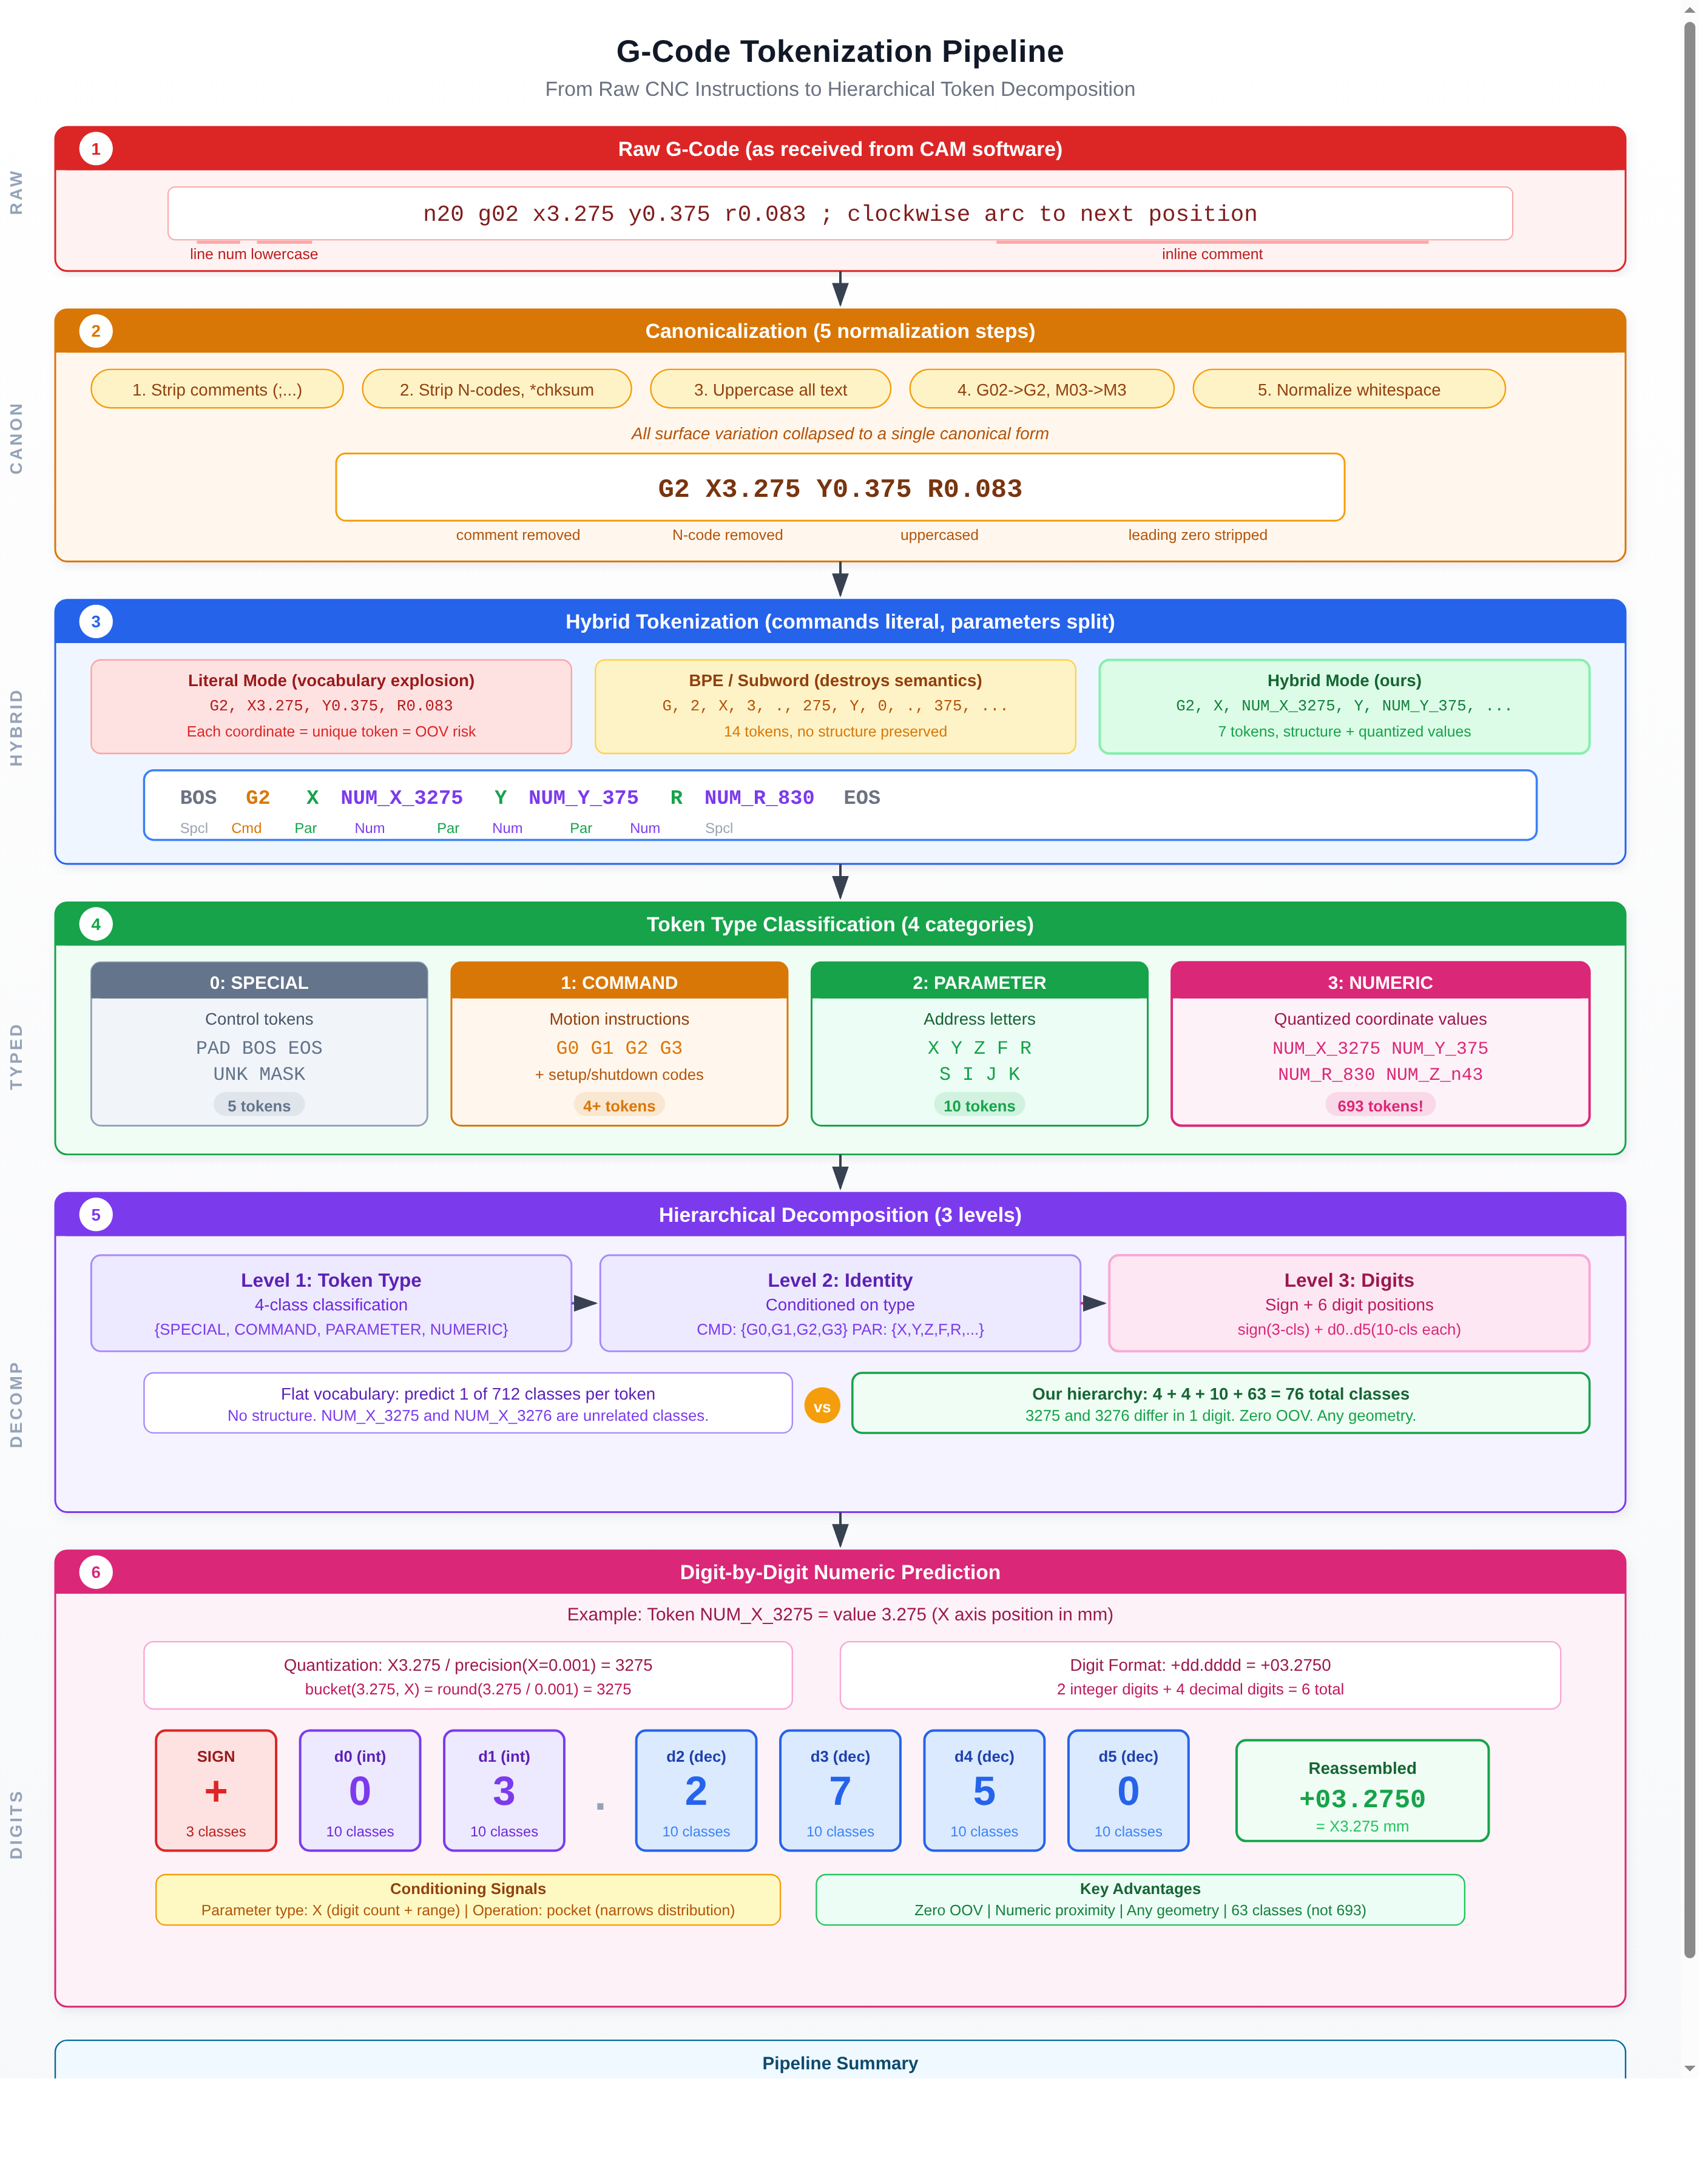
\includegraphics[width=0.95\textwidth, trim=0 280 0 0, clip]{figures/gcode_tokenization_pipeline.png}
\caption{End-to-end tokenization pipeline. Raw G-code is canonicalized (5~steps), split into typed hybrid tokens, classified into 4~categories, decomposed hierarchically (3~levels), and predicted digit-by-digit (sign + 6~digits).}
\label{fig:pipeline}
\end{figure}

\begin{figure}[htbp]
\centering
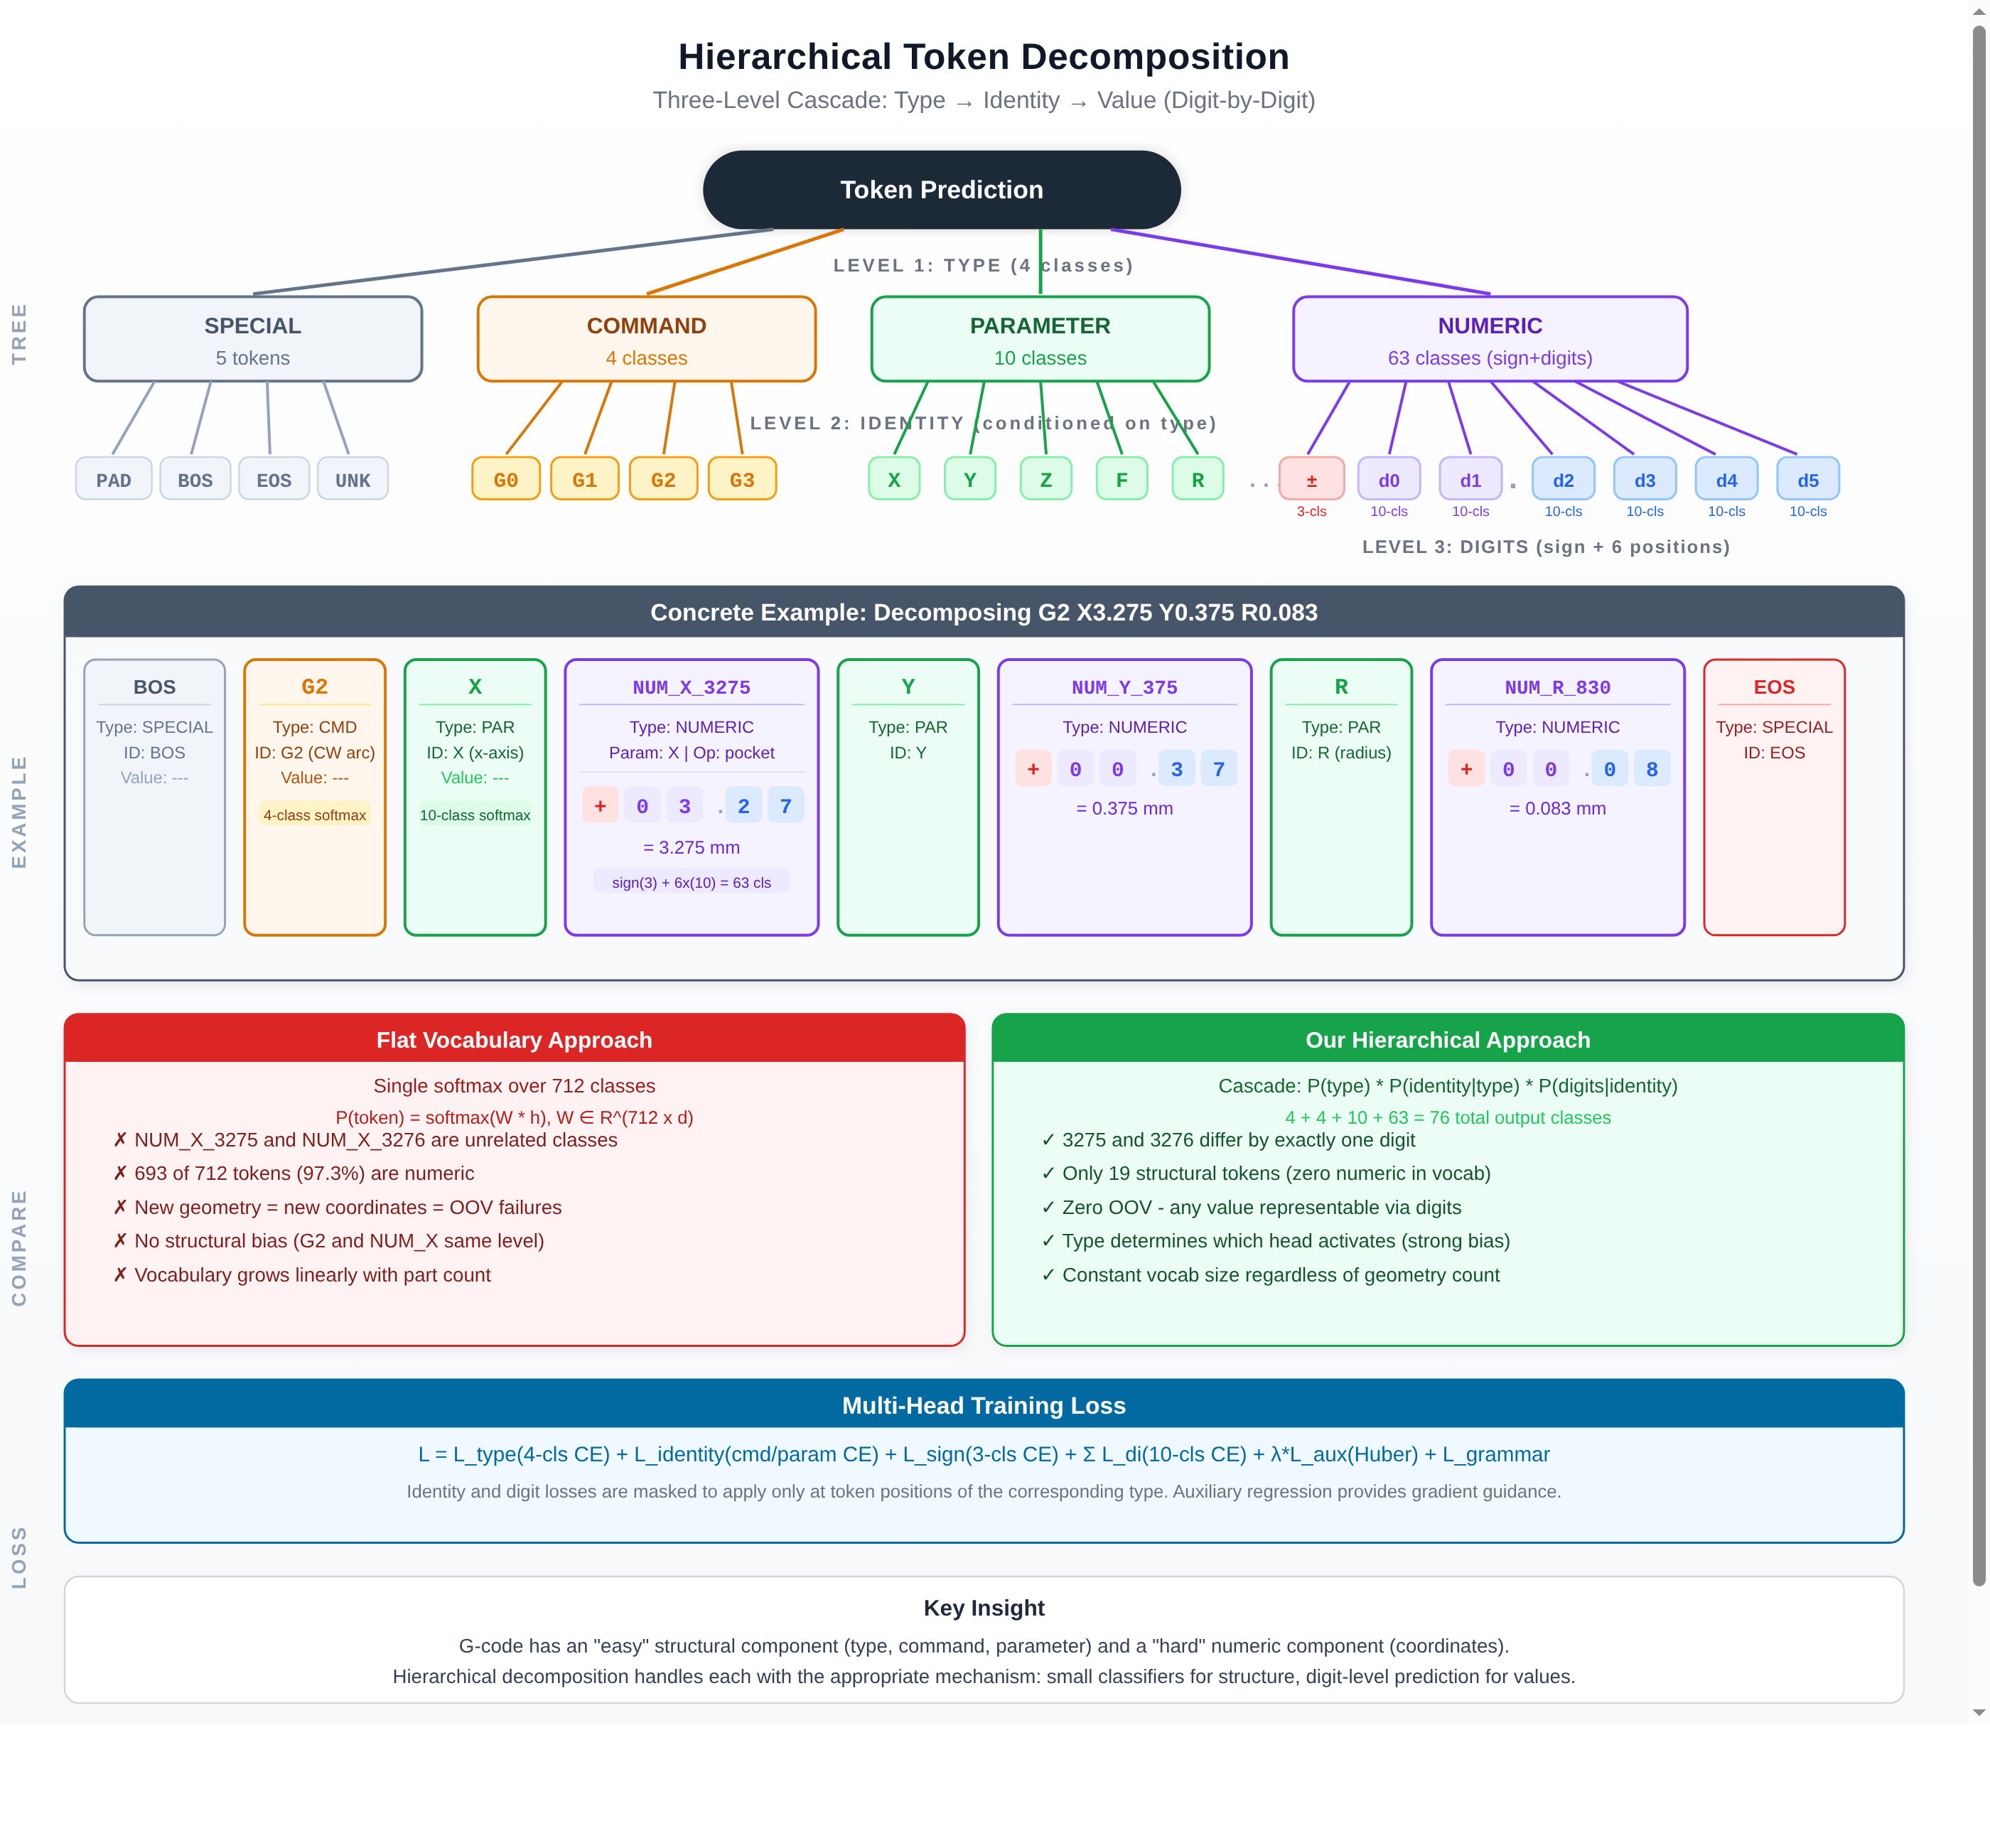
\includegraphics[width=0.95\textwidth, trim=0 1100 0 0, clip]{figures/hierarchical_decomposition.png}
\caption{Hierarchical token decomposition. Top: three-level cascade (type $\to$ identity $\to$ digits) with cardinality at each branch. Bottom: concrete decomposition of \texttt{G2 X3.275 Y0.375 R0.083} showing type, identity, and digit predictions for each token.}
\label{fig:decomposition_detail}
\end{figure}

\end{document}
